% Memoria del trabajo. Compilar (desde esta carpeta):   tectonic -X compile memoria.tex
\documentclass[11pt,a4paper,twoside,openany]{report}
% Preámbulo común de la memoria y de la guía de uso.
% Tipografía: Libertinus (texto y matemáticas), cuerpo 11 pt, interlineado holgado. Compilar con Tectonic o XeLaTeX.

\usepackage[spanish,es-noshorthands,es-tabla,es-nodecimaldot]{babel}
\usepackage{libertinus}
\usepackage{microtype}
\usepackage[a4paper,top=2.7cm,bottom=2.7cm,inner=2.8cm,outer=2.4cm,headheight=15pt]{geometry}
\linespread{1.13}
\clubpenalty=10000
\widowpenalty=10000
\displaywidowpenalty=10000
\raggedbottom
\emergencystretch=2.5em
\tolerance=1200
\hbadness=3000

\usepackage{amsmath}
\usepackage{etoolbox}
\usepackage{xcolor}
\usepackage{graphicx}
\usepackage{placeins}
\usepackage{float}
\usepackage{caption}
\usepackage{subcaption}
\usepackage{booktabs,tabularx,array,multirow,makecell}
\usepackage{enumitem}
\usepackage{needspace}
\usepackage{fancyhdr}
\usepackage{titlesec}
\usepackage{listings}
\usepackage{tikz}
\usetikzlibrary{arrows.meta,positioning,shapes.geometric,fit,calc}
\usepackage{algorithm}
\usepackage{algpseudocode}
\usepackage[hidelinks,bookmarksnumbered]{hyperref}

% ── Colores (los mismos de las figuras y de la web) ──
\definecolor{azul}{HTML}{2A78D6}
\definecolor{naranja}{HTML}{EB6834}
\definecolor{aqua}{HTML}{1BAF7A}
\definecolor{amarillo}{HTML}{EDA100}
\definecolor{rosa}{HTML}{E87BA4}
\definecolor{verde}{HTML}{008300}
\definecolor{violeta}{HTML}{6250D6}
\definecolor{rojo}{HTML}{E34948}
\definecolor{gris}{HTML}{52514E}
\definecolor{grisclaro}{HTML}{F1F0EC}
\definecolor{tinta}{HTML}{14203A}

% ── Títulos: cada capítulo empieza en página nueva; los apartados no se quedan huérfanos al pie de la página ──
\titleformat{\chapter}[display]{\normalfont\bfseries\color{tinta}}{\large\scshape\color{gris}Capítulo \thechapter}{0.35em}{\Huge}[\vspace{0.4em}\titlerule]
\titlespacing*{\chapter}{0pt}{-10pt}{26pt}
\titleformat{\section}{\normalfont\Large\bfseries\color{tinta}}{\thesection}{0.7em}{}
\titlespacing*{\section}{0pt}{2.0ex plus 0.4ex}{1.1ex plus 0.2ex}
\titleformat{\subsection}{\normalfont\large\bfseries\color{tinta}}{\thesubsection}{0.7em}{}
\titlespacing*{\subsection}{0pt}{1.7ex plus 0.3ex}{0.8ex plus 0.2ex}
\titleformat{\subsubsection}{\normalfont\normalsize\bfseries\itshape\color{gris}}{}{0pt}{}
\titlespacing*{\subsubsection}{0pt}{1.3ex plus 0.2ex}{0.5ex plus 0.1ex}
% Si queda menos de ~28 % de página, el apartado empieza en la página siguiente (así no se parte por la mitad)
\pretocmd{\chapter}{\FloatBarrier}{}{}
\pretocmd{\section}{\Needspace{0.40\textheight}}{}{}
\pretocmd{\subsection}{\Needspace{0.22\textheight}}{}{}
\pretocmd{\subsubsection}{\Needspace{0.10\textheight}}{}{}

% ── Cabecera y pie ──
\pagestyle{fancy}
\fancyhf{}
\fancyhead[LE]{\small\slshape\leftmark}
\fancyhead[RO]{\small\slshape\rightmark}
\fancyfoot[C]{\small\thepage}
\renewcommand{\headrulewidth}{0.3pt}
\renewcommand{\chaptermark}[1]{\markboth{#1}{}}
\renewcommand{\sectionmark}[1]{\markright{\thesection\ \ #1}}
\fancypagestyle{plain}{\fancyhf{}\fancyfoot[C]{\small\thepage}\renewcommand{\headrulewidth}{0pt}}

% ── Figuras, tablas y listas ──
\captionsetup{font=small,labelfont=bf,labelsep=period,justification=centering,format=plain}
\captionsetup[table]{position=above,skip=6pt}
\captionsetup[figure]{position=below,skip=6pt}
\setlist{itemsep=0.25em,topsep=0.4em,parsep=0pt}
\renewcommand{\arraystretch}{1.18}
\graphicspath{{figuras/}{../web/capturas/}{capturas/}}
\renewcommand{\topfraction}{0.88}\renewcommand{\bottomfraction}{0.7}\renewcommand{\textfraction}{0.12}\renewcommand{\floatpagefraction}{0.65}\setcounter{topnumber}{3}\setcounter{totalnumber}{5}
\setcounter{tocdepth}{2}
\setcounter{secnumdepth}{3}

% ── Pseudocódigo en español ──
\floatname{algorithm}{Algoritmo}
\renewcommand{\listalgorithmname}{Lista de algoritmos}
\algrenewcommand\algorithmicrequire{\textbf{Entrada:}}
\algrenewcommand\algorithmicensure{\textbf{Salida:}}
\algrenewcommand\algorithmicwhile{\textbf{mientras}}
\algrenewcommand\algorithmicdo{\textbf{hacer}}
\algrenewcommand\algorithmicfor{\textbf{para}}
\algrenewcommand\algorithmicforall{\textbf{para cada}}
\algrenewcommand\algorithmicif{\textbf{si}}
\algrenewcommand\algorithmicthen{\textbf{entonces}}
\algrenewcommand\algorithmicelse{\textbf{si no}}
\algrenewcommand\algorithmicrepeat{\textbf{repetir}}
\algrenewcommand\algorithmicuntil{\textbf{hasta que}}
\algrenewcommand\algorithmicreturn{\textbf{devolver}}
\algrenewtext{EndWhile}{\textbf{fin mientras}}
\algrenewtext{EndFor}{\textbf{fin para}}
\algrenewtext{EndIf}{\textbf{fin si}}
\algrenewtext{Else}{\textbf{si no}}
\algrenewtext{ElsIf}[1]{\textbf{si no, si} #1 \textbf{entonces}}
\algrenewtext{Procedure}[2]{\textbf{procedimiento} \textsc{#1}(#2)}
\algrenewtext{EndProcedure}{\textbf{fin procedimiento}}
\algrenewcommand\alglinenumber[1]{\footnotesize\color{gris}#1}
\newcommand{\Comentario}[1]{\hfill\textcolor{gris}{\small\textit{#1}}}

% ── Código y comandos ──
\lstset{basicstyle=\ttfamily\small,breaklines=true,breakatwhitespace=false,columns=fullflexible,keepspaces=true,frame=single,rulecolor=\color{grisclaro},
        backgroundcolor=\color{grisclaro},xleftmargin=0.4em,xrightmargin=0.4em,aboveskip=0.8em,belowskip=0.6em,showstringspaces=false,
        inputencoding=utf8,extendedchars=true,literate={á}{{\'a}}1 {é}{{\'e}}1 {í}{{\'i}}1 {ó}{{\'o}}1 {ú}{{\'u}}1 {ñ}{{\~n}}1 {Á}{{\'A}}1 {É}{{\'E}}1 {Ó}{{\'O}}1 {¿}{{?`}}1 {¡}{{!`}}1 {→}{{$\rightarrow$}}1}
\newcommand{\cod}[1]{\texttt{\small #1}}
\newcommand{\Oh}[1]{\ensuremath{O\!\left(#1\right)}}

% ── Cuadros destacados ──
\newcommand{\recuadro}[2]{\par\vspace{0.6em}\noindent\begin{minipage}{\linewidth}\noindent\colorbox{grisclaro}{\parbox{\dimexpr\linewidth-2\fboxsep}{\small\textbf{#1.} #2}}\end{minipage}\par\vspace{0.6em}}

% ── Datos de portada ──
\newcommand{\titulotrabajo}{El problema del viajante sobre la red de carreteras de España}
\newcommand{\subtitulotrabajo}{Construcción del grafo vial, algoritmos exactos, heurísticos y metaheurísticos, y estudio empírico de su complejidad}
\newcommand{\autorestrabajo}{Raimundo, Pablo, Juan y Jiahao}
\newcommand{\asignatura}{Asignatura MATI \textperiodcentered\ Curso 2026--27}
\newcommand{\fechatrabajo}{Noviembre de 2026}

% Formato de los capítulos de los apéndices (se activa tras ppendix)
\newcommand{\apendicestyle}{\titleformat{\chapter}[display]{\normalfont\bfseries\color{tinta}}{\large\scshape\color{gris}Apéndice \thechapter}{0.35em}{\Huge}[\vspace{0.4em}\titlerule]}


\hypersetup{pdftitle={El problema del viajante sobre la red de carreteras de España},pdfauthor={Raimundo, Pablo, Juan y Jiahao},pdfsubject={Memoria del trabajo de MATI},pdflang={es}}

\begin{document}
\pagenumbering{roman}
\begin{titlepage}
  \thispagestyle{empty}
  \centering
  \vspace*{2.2cm}
  {\large\scshape\color{gris}\asignatura\par}
  \vspace{2.4cm}
  {\fontsize{26}{32}\selectfont\bfseries\color{tinta}\titulotrabajo\par}
  \vspace{1.0cm}
  {\large\itshape\color{gris}\subtitulotrabajo\par}
  \vspace{2.2cm}
  \begin{tikzpicture}
    \draw[line width=0.8pt,color=azul] (0,0) -- (6.0,0);
    \foreach \x/\c in {0/azul,1.2/naranja,2.4/aqua,3.6/violeta,4.8/rojo,6.0/verde} {\fill[\c] (\x,0) circle (3.2pt);}
  \end{tikzpicture}
  \vspace{2.4cm}

  {\Large\autorestrabajo\par}
  \vfill
  {\large\fechatrabajo\par}
  \vspace{1.0cm}
  {\small\color{gris}Código, datos y web del trabajo: repositorio \texttt{MATI\_TRABAJO} en GitHub\par}
\end{titlepage}

\chapter*{Resumen}
\addcontentsline{toc}{chapter}{Resumen}
\markboth{Resumen}{}
Este trabajo estudia el \emph{problema del viajante} (TSP) sobre la red de carreteras real de la España peninsular. Partimos de un
extracto de OpenStreetMap, del que construimos un grafo vial simplificado y fuertemente conexo con 179.594 nodos y 309.250 aristas dirigidas.
A partir de él calculamos, para 75 ciudades (las 47 capitales de provincia peninsulares y 28 municipios de más de 100.000 habitantes),
tablas de distancias por camino mínimo que dan lugar a 480 versiones del problema (240 grafos de ciudades distintos), según el tipo de carreteras,
la medida (kilómetros o tiempo de viaje), el sentido de las vías y el ámbito geográfico.

Implementamos ocho algoritmos que cubren las familias clásicas: tres exactos (fuerza bruta, Held--Karp y DFJ), tres heurísticos o aproximados (vecino más
cercano, 2-opt y Christofides) y dos metaheurísticas (recocido simulado y algoritmo genético). Los comparamos en un estudio empírico de
4.706 ejecuciones sobre las 240 versiones y sobre subconjuntos aleatorios de 5 a 75 ciudades, midiendo tiempo, memoria y desviación respecto al óptimo,
y contrastamos la complejidad teórica con la observada en notación~$O$.

Los resultados muestran que los exactos de enumeración crecen de forma exponencial (la fuerza bruta se agota en 11 ciudades y Held--Karp, por memoria, en
unas 20), mientras que la programación entera (DFJ) resuelve las 75 ciudades al óptimo en unos 4~s; que el 2-opt ofrece la mejor relación entre calidad
(1--5~\% sobre el óptimo) y tiempo (milisegundos); y que el tipo de red y el sentido de las vías modifican el óptimo tanto como la elección del algoritmo.
Completan el trabajo una web interactiva que anima los algoritmos sobre el mapa y una guía de uso para el equipo.

\vspace{1.2em}
\noindent\textbf{Palabras clave:} problema del viajante, OpenStreetMap, grafos, algoritmos exactos, heurísticas, metaheurísticas, complejidad computacional.

\chapter*{Abstract}
\addcontentsline{toc}{chapter}{Abstract}
\markboth{Abstract}{}
\begin{otherlanguage}{english}
This work studies the \emph{travelling salesman problem} (TSP) on the real road network of mainland Spain. From an OpenStreetMap extract we build a simplified,
strongly connected road graph with 179,594 nodes and 309,250 directed edges. For 75 cities (the 47 mainland provincial capitals plus 28 municipalities with
over 100,000 inhabitants) we compute shortest-path distance tables that give rise to 480 problem versions (240 distinct city graphs), depending on road type,
cost measure (kilometres or travel time), one-way handling and geographic scope.

We implement eight algorithms covering the classical families: three exact (brute force, Held--Karp and DFJ integer programming), three heuristic or
approximation algorithms (nearest neighbour, 2-opt and Christofides) and two metaheuristics (simulated annealing and a genetic algorithm). An empirical
study of 4,706 runs over the 240 versions and over random subsets of 5 to 75 cities measures time, memory and deviation from the optimum, and compares
theoretical with observed complexity in $O$ notation. Enumeration-based exact methods grow exponentially, whereas integer programming solves all 75 cities
to optimality in about 4~s; 2-opt gives the best quality--time trade-off. An interactive web application animating the algorithms on the map and a user guide complete the work.
\end{otherlanguage}
\clearpage

\tableofcontents
\clearpage\pagenumbering{arabic}
\chapter{Introducción}\label{cap:intro}

\section{El problema del viajante}

El \emph{problema del viajante} (en inglés, \emph{travelling salesman problem}, TSP) es uno de los problemas clásicos de la optimización
combinatoria. Un viajante debe visitar un conjunto de ciudades, pasando por cada una exactamente una vez, y volver a la ciudad de partida
recorriendo la menor distancia posible. Aunque el enunciado es sencillo, encontrar la mejor ruta es difícil: con $n$ ciudades hay $(n-1)!$ recorridos
posibles, un número que crece más deprisa que cualquier exponencial.

Formalmente, sea $V=\{0,1,\dots,n-1\}$ el conjunto de ciudades y $c(i,j)\ge 0$ el coste de ir de la ciudad $i$ a la ciudad $j$. Una ruta es una permutación
$\pi$ de $V$ y su coste, incluida la vuelta al inicio, es
\begin{equation}\label{eq:coste}
  C(\pi)\;=\;\sum_{k=0}^{n-2} c\bigl(\pi_k,\pi_{k+1}\bigr)\;+\;c\bigl(\pi_{n-1},\pi_0\bigr).
\end{equation}
El problema consiste en encontrar la permutación $\pi^{*}$ que minimiza $C(\pi)$. Si $c(i,j)=c(j,i)$ para todo par de ciudades el problema es
\emph{simétrico}; en caso contrario es \emph{asimétrico}. Si además se cumple la \emph{desigualdad triangular},
\begin{equation}\label{eq:triangular}
  c(i,k)\;\le\;c(i,j)+c(j,k)\qquad\text{para todo }i,j,k\in V,
\end{equation}
decimos que el problema es \emph{métrico}; esta propiedad es necesaria para algunas garantías de aproximación, como la del algoritmo de Christofides
(sección~\ref{sec:christofides}).

El TSP es un problema NP-difícil~\cite{karp1972,garey1979}: no se conoce ningún algoritmo que lo resuelva en tiempo polinómico en el caso
general, y se cree que no existe. Eso no significa que sea imposible resolverlo en la práctica. Los algoritmos exactos modernos, basados en programación
entera, han resuelto instancias de decenas de miles de ciudades~\cite{applegate2006}, y las heurísticas obtienen soluciones muy buenas en
tiempos pequeños. La cuestión interesante es \emph{cuánto cuesta} cada enfoque y \emph{qué se sacrifica} a cambio de rapidez, que es lo que estudia
este trabajo.

\section{Motivación: carreteras reales}

La mayoría de los estudios sobre el TSP usan instancias sintéticas (puntos en el plano con distancia euclídea) o colecciones clásicas. Aquí lo
planteamos sobre un caso real: \emph{las ciudades de España y las carreteras que las unen}. Esto añade tres ingredientes que no aparecen en el plano:
\begin{itemize}
  \item \textbf{Las distancias son por carretera}, es decir, caminos mínimos sobre un grafo vial con cientos de miles de nodos, no distancias en línea recta.
  \item \textbf{Hay vías de sentido único} (por ejemplo, las dos calzadas de una autovía son aristas distintas), de modo que ir de $A$ a $B$ puede costar distinto que de $B$ a $A$.
        El problema es entonces asimétrico, y la elección entre un modelo dirigido y otro no dirigido pasa a ser parte del estudio.
  \item \textbf{Se puede medir en kilómetros o en tiempo}, y la ruta más corta no tiene por qué ser la más rápida.
\end{itemize}

Estos ingredientes permiten, además, plantear preguntas que un benchmark sintético no permite: ¿cómo cambia el recorrido óptimo si solo se pueden usar autovías?
¿Cuánto cuesta ignorar los sentidos únicos? ¿Qué algoritmos se pueden aplicar a qué versión del problema, y por qué?

\section{Objetivos}

El objetivo general es \textbf{medir cómo mejoran en complejidad y en tiempo los distintos algoritmos del viajante al buscar una solución óptima o completa, y qué
se pierde en calidad cuando se renuncia al óptimo}. Lo desglosamos en cinco preguntas, que guían todo el estudio:
\begin{enumerate}[label=\textbf{P\arabic*.}]
  \item ¿Qué algoritmo puede usarse con qué versión del grafo, y por qué?
  \item ¿Cómo crecen el tiempo y la memoria con el número de ciudades? ¿Coincide con la complejidad teórica?
  \item ¿Cuánto se aleja de la ruta óptima cada algoritmo que no garantiza el óptimo?
  \item ¿Cómo cambian los resultados con el tipo de carreteras, el peso (kilómetros o tiempo) y el sentido de las vías?
  \item ¿Qué algoritmo conviene en cada caso, atendiendo a calidad y tiempo?
\end{enumerate}
Para responderlas hay que resolver antes problemas previos de ingeniería de datos: obtener un grafo vial fiable, elegir y justificar un conjunto de ciudades, y
definir un conjunto de \emph{versiones} del problema bien especificadas y reproducibles.

\section{Qué se ha hecho}

El trabajo se organiza en cinco partes encadenadas (figura~\ref{fig:pipeline}), a las que se suman una web interactiva y esta memoria:
\begin{enumerate}[label=\textbf{Parte \arabic*.},leftmargin=*,labelsep=0.5em]
  \item \textbf{Construcción del grafo.} Descarga de un extracto de OpenStreetMap, filtrado, simplificación y asignación de longitudes y tiempos (capítulo~\ref{cap:grafo}).
  \item \textbf{Ciudades y versiones del grafo.} Selección de 75 ciudades y cálculo de tablas de distancias que originan 480 versiones del problema (capítulo~\ref{cap:versiones}).
  \item \textbf{Algoritmos.} Implementación de ocho algoritmos, tres exactos, tres heurísticos y dos metaheurísticos (capítulo~\ref{cap:algoritmos}).
  \item \textbf{Estudio empírico.} Ejecución sistemática de los algoritmos y análisis de tiempo, memoria y calidad (capítulos~\ref{cap:metodologia} y~\ref{cap:resultados}).
  \item \textbf{Conclusiones.} Respuesta a las preguntas planteadas y recomendaciones de uso (capítulo~\ref{cap:conclusiones}).
\end{enumerate}

\begin{figure}[htbp]
  \centering
  \begin{tikzpicture}[
      caja/.style={draw=#1!70!black,fill=#1!10,rounded corners=3pt,align=center,minimum height=1.25cm,text width=2.9cm,font=\small,line width=0.6pt},
      flecha/.style={-{Stealth[length=2.2mm]},line width=0.7pt,color=gris}]
    \node[caja=azul] (a) {\textbf{OpenStreetMap}\\extracto de España\\(\texttt{.osm.pbf}, 1,4~GB)};
    \node[caja=naranja,right=0.75cm of a] (b) {\textbf{Grafo vial}\\179.594 nodos\\309.250 aristas};
    \node[caja=aqua,right=0.75cm of b] (c) {\textbf{Versiones}\\16 tablas de distancias\\240 grafos de ciudades};
    \node[caja=violeta,below=0.95cm of c] (d) {\textbf{8 algoritmos}\\exactos, heurísticos,\\metaheurísticas};
    \node[caja=rojo,left=0.75cm of d] (e) {\textbf{Estudio empírico}\\4.706 ejecuciones\\tiempo, memoria, calidad};
    \node[caja=verde,left=0.75cm of e] (f) {\textbf{Conclusiones}\\y recomendaciones\\de uso};
    \node[caja=amarillo,below=0.9cm of e] (g) {\textbf{Web interactiva}\\animación paso a paso\\y carrera};
    \draw[flecha] (a) -- (b); \draw[flecha] (b) -- (c); \draw[flecha] (c) -- (d); \draw[flecha] (d) -- (e); \draw[flecha] (e) -- (f);
    \draw[flecha,dashed] (d) |- (g.east);
  \end{tikzpicture}
  \caption{Esquema del trabajo: de los datos de OpenStreetMap a las conclusiones. La web reutiliza los datos y los algoritmos.}
  \label{fig:pipeline}
\end{figure}

\section{Herramientas y reproducibilidad}

Todo el trabajo está escrito en Python~3 y se entrega como un \emph{notebook} (\texttt{trabajo\_tsp.ipynb}) más tres scripts de apoyo (los \emph{anexos}):
el Anexo~A descarga el extracto, el Anexo~B construye el grafo y el Anexo~C ejecuta el estudio empírico en paralelo. Usamos NetworkX~\cite{hagberg2008}
para los grafos, NumPy~\cite{harris2020} y SciPy~\cite{virtanen2020} para el cálculo numérico, PuLP con el \emph{solver} CBC para la programación entera
de DFJ y OSMnx~\cite{boeing2017} únicamente en la construcción del grafo. El código, los datos intermedios y los resultados se versionan en GitHub, y cada
resultado de esta memoria se puede regenerar con los comandos del apéndice~\ref{ap:reproducir}.

\section{Estructura de la memoria}

El capítulo~\ref{cap:grafo} describe los datos y la construcción del grafo vial. El capítulo~\ref{cap:versiones} presenta las ciudades y las versiones del problema.
El capítulo~\ref{cap:algoritmos} explica los ocho algoritmos y justifica su elección. El capítulo~\ref{cap:metodologia} detalla la metodología del estudio y el
capítulo~\ref{cap:resultados} presenta sus resultados. El capítulo~\ref{cap:conclusiones} recoge las conclusiones. El capítulo~\ref{cap:web} describe la web interactiva
y el capítulo~\ref{cap:organizacion} la organización del trabajo en equipo, el uso de herramientas de inteligencia artificial y los problemas encontrados. Los apéndices
reúnen las instrucciones para reproducir el trabajo y material complementario.

\chapter{Datos y construcción del grafo vial}\label{cap:grafo}

Este capítulo explica de dónde salen las carreteras, cómo se convierten en un grafo utilizable por los algoritmos y qué decisiones de diseño se tomaron en el
camino, incluidas las que no funcionaron.

\section{Fuente de los datos}

Las carreteras proceden de \emph{OpenStreetMap} (OSM)~\cite{haklay2008}, una base de datos geográfica colaborativa publicada bajo la licencia ODbL (\emph{Open Database License}), que obliga a citar la
fuente como «\textcopyright\ OpenStreetMap contributors». No es una fuente oficial: la calidad de los datos depende de la comunidad de mapeadores, lo que implica
que algunas etiquetas (por ejemplo, la velocidad máxima de un tramo) están incompletas. Aceptamos esta limitación porque OSM es la única fuente abierta que describe toda la red
con la topología necesaria (tramos, sentidos de circulación y jerarquía de las vías).

Usamos el extracto de España de \emph{Geofabrik} (\texttt{spain-latest.osm.pbf}, 1,4~GB, última modificación el 19 de octubre de 2026). Para las ciudades empleamos datos oficiales del INE
(capítulo~\ref{cap:versiones}).

\section{Un primer enfoque descartado: la API Overpass}

El primer enfoque fue descargar la red directamente con OSMnx~\cite{boeing2017} a través de la API pública \emph{Overpass}, dividiendo España en 324 consultas. En unas once horas solo se completaron
19 consultas (el 6~\%), por errores \texttt{ConnectTimeout} y \texttt{502 Bad Gateway} del servidor público, que estaba saturado; además, una de sus dos direcciones IP no aceptaba conexiones y
OSMnx fija una sola IP por servidor. Estimamos que completar la descarga llevaría días y no sería reproducible. Se conserva el registro de aquel intento como evidencia
(\texttt{docs/intento\_overpass/}), pero se descartó.

\recuadro{Decisión}{Sustituir Overpass por un único archivo descargable y reanudable (el extracto de Geofabrik) y filtrarlo en local. La descarga completa tarda unos siete minutos y puede repetirse.}

\section{Filtrado y construcción del grafo}\label{sec:construccion}

El extracto de 1,4~GB contiene todos los elementos de OSM de España. Nos interesa solo la red de carreteras de coche, así que conservamos las vías cuya etiqueta
\texttt{highway} es \texttt{motorway} (autopista y autovía), \texttt{trunk} (vía rápida), \texttt{primary} (red principal) o \texttt{secondary} (red secundaria), junto con sus
enlaces (\texttt{*\_link}). El filtrado se hace con la biblioteca \texttt{pyosmium} en dos pasadas: la primera selecciona las vías que cumplen el filtro; la segunda recupera las coordenadas de los nodos que esas vías usan.

El grafo resultante es un \emph{multigrafo dirigido}: cada tramo de carretera de doble sentido se representa con dos aristas, una en cada dirección, y una autovía con
calzadas separadas son dos aristas distintas. Se admite más de una arista entre el mismo par de nodos (carreteras paralelas), que se distinguen por una clave.

\subsection{Simplificación}

Un grafo con todos los puntos del trazado tendría millones de nodos. Se \emph{simplifica}: solo se conservan como nodos las intersecciones y los extremos de carretera, y cada arista
representa un tramo completo entre dos de ellos, con su longitud total. Seguimos las mismas reglas que OSMnx: un nodo se conserva si tiene bucle sobre sí mismo, si no tiene aristas
de entrada o de salida, o si no es un simple punto intermedio (un nodo con exactamente dos vecinos y grado 2 o 4 se considera intermedio y se fusiona). La longitud de un tramo es la suma de los segmentos
originales, medidos con la distancia ortodrómica (\emph{great-circle}) entre coordenadas.

\subsection{Conectividad}

Para que exista un camino entre cualquier par de nodos, se conserva la mayor componente \emph{fuertemente conexa} del grafo, es decir, aquella donde se puede ir de cualquier nodo a cualquier otro respetando
los sentidos de circulación. Esto elimina también los fragmentos aislados (islas, tramos desconectados, extremos de frontera). El grafo base final es fuertemente conexo y cubre únicamente la
\textbf{España peninsular}: Baleares, Canarias, Ceuta y Melilla no están.

\section{Atributos del grafo}

Cada arista guarda tres valores numéricos y varios descriptivos. La velocidad se toma de la etiqueta \texttt{maxspeed} de OSM cuando existe; si falta, se imputa la media de los tramos
de su mismo tipo de vía. Con la longitud $L$ en metros y la velocidad $v$ en km/h, el tiempo de viaje en segundos es
\begin{equation}\label{eq:tiempo}
  t\;=\;\frac{L}{v/3{,}6}.
\end{equation}
Por ejemplo, un tramo de la AP-8 de $5.895{,}57$~m a $100$~km/h tiene un tiempo de $212{,}24$~s. La tabla~\ref{tab:atributos} resume los atributos.

\begin{table}[htbp]
  \centering
  \caption{Atributos de las aristas del grafo base.}\label{tab:atributos}
  \small
  \begin{tabularx}{\linewidth}{@{}l l c X@{}}
    \toprule
    Atributo & Tipo & Presencia & Significado \\
    \midrule
    \texttt{length} & decimal & 100 \% & Longitud del tramo en metros (peso para distancias). \\
    \texttt{travel\_time} & decimal & 100 \% & Tiempo de viaje en segundos, según la ecuación~\eqref{eq:tiempo} (peso para tiempos). \\
    \texttt{speed\_kph} & decimal & 100 \% & Velocidad usada (km/h): la máxima de OSM o la media de su tipo de vía. \\
    \texttt{highway} & texto & 100 \% & Tipo de vía (\texttt{motorway}, \texttt{trunk}, \texttt{primary}, \texttt{secondary} o sus enlaces). \\
    \texttt{oneway} & booleano & 100 \% & \texttt{True} si es de sentido único (227.446 aristas) o \texttt{False} si es de doble sentido (81.804). \\
    \texttt{ref} & texto & 90,3 \% de los km & Código de la carretera (\texttt{AP-7}, \texttt{A-4}, \texttt{N-340}\dots). \\
    \texttt{name} & texto & 72,0 \% de los km & Nombre en lenguaje natural («Autovía del Mediterráneo»). \\
    \bottomrule
  \end{tabularx}
\end{table}

Los nodos guardan su longitud (\texttt{x}), su latitud (\texttt{y}) y el número de calles que confluyen (\texttt{street\_count}). OSM no nombra las intersecciones, por lo que
\emph{los nodos no tienen nombre}: los nombres de ciudad se asocian a un nodo en el capítulo~\ref{cap:versiones}.

Para poder guardar el grafo en un formato estándar se eliminaron dos atributos de OSM: \texttt{osmid} (listas de identificadores, inútiles para trabajar y no admitidas por el formato) y
\texttt{maxspeed} (con listas y valores no numéricos como \texttt{ES:urban} o \texttt{50 mph}, cuya información ya está resuelta en \texttt{speed\_kph}). Los atributos
que OSM da como lista (\texttt{ref}, \texttt{name}) se unieron en un único texto.

\subsection{Formato de archivo}

El grafo se guarda en \emph{GraphML}, un formato estándar de grafos basado en XML, con \texttt{nx.write\_graphml} de NetworkX. Este formato declara el tipo real de cada atributo,
de modo que al leerlo con \texttt{nx.read\_graphml} los números llegan como números y los booleanos como booleanos, y el \emph{notebook} solo necesita NetworkX, como las prácticas de la asignatura.
El archivo ocupa 108~MB y se carga en unos 20 segundos.

\section{Descripción del grafo obtenido}

El grafo base tiene \textbf{179.594 nodos} y \textbf{309.250 aristas dirigidas} (unos 183.000~km contando cada sentido). Hay 3.349 pares de nodos unidos por más de una arista.
La tabla~\ref{tab:tipos} reparte las aristas por tipo de vía y la tabla~\ref{tab:nodos} clasifica los nodos según el número de calles que confluyen.

\begin{table}[htbp]
  \centering
  \caption{Aristas y kilómetros por tipo de vía.}\label{tab:tipos}
  \small
  \begin{tabularx}{0.92\linewidth}{@{}l X r r@{}}
    \toprule
    Tipo (\texttt{highway}) & Qué es & Aristas & Km \\
    \midrule
    \texttt{motorway} & autopista y autovía & 17.618 & 31.485 \\
    \texttt{trunk} & vía rápida o carretera desdoblada & 52.029 & 31.438 \\
    \texttt{primary} & carretera de la red principal & 75.467 & 40.454 \\
    \texttt{secondary} & carretera de la red secundaria & 100.495 & 69.150 \\
    \texttt{*\_link} & enlaces y accesos de los cuatro anteriores & 63.641 & 10.233 \\
    \midrule
    \multicolumn{2}{@{}l}{\textbf{Total}} & \textbf{309.250} & \textbf{182.760} \\
    \bottomrule
  \end{tabularx}
\end{table}

\begin{table}[htbp]
  \centering
  \caption{Tipos de nodo según el número de calles que confluyen (\texttt{street\_count}).}\label{tab:nodos}
  \small
  \begin{tabularx}{0.92\linewidth}{@{}c X r@{}}
    \toprule
    Calles & Significado típico & Nodos \\
    \midrule
    1 & extremos (fin de carretera o corte en la frontera) & 1.058 \\
    2 & empalmes entre dos vías distintas de OSM & 4.612 \\
    3 & bifurcaciones o incorporaciones (entradas y salidas de autovía) & 161.516 \\
    4 & cruces de cuatro ramas & 10.332 \\
    5 o más & nudos complejos & 2.076 \\
    \bottomrule
  \end{tabularx}
\end{table}

\section{Memoria y rendimiento: reescribir la simplificación}

El grafo con carreteras secundarias no cabía en memoria con el flujo habitual de OSMnx (\texttt{graph\_from\_*}): se estimaban unos 12~GB y el proceso fue finalizado por el sistema operativo por falta
de memoria. En lugar de eso, el Anexo~B reimplementa con \emph{arrays} de NumPy las reglas de simplificación de OSMnx, sin construir un grafo gigante de NetworkX intermedio. El pico de memoria medido es de
unos 2,2~GB y la construcción completa tarda unos cuatro minutos.

Para asegurarnos de que la reimplementación es fiel, la comparamos con el grafo \emph{ligero} (solo \texttt{motorway}, \texttt{trunk}, \texttt{primary} y sus enlaces) que ya habíamos construido con el método anterior:
los dos tienen los mismos 108.050 nodos (con los mismos identificadores), las mismas 181.006 aristas y las mismas longitudes (110.128,4~km). Solo cambian ligeramente las velocidades imputadas (diferencia media de
0,05~km/h; 136 aristas difieren más de 1~km/h), porque el método anterior elegía de forma arbitraria el tipo de vía de las aristas mixtas y el nuevo usa el de mayor jerarquía.

\section{Por qué incluir las carreteras secundarias}

El grafo base incluye carreteras secundarias; el ligero no. Con solo autopistas, vías rápidas y red principal, una red \emph{sin autovías} queda llena de agujeros: Almería quedaba a 142~km de la red, y la ruta
Madrid--Sevilla medía 761~km en lugar de unos 510. Con las secundarias el resultado es utilizable, y además las ciudades vecinas quedan mucho más cerca entre sí (en la red sin secundarias, Terrassa--Sabadell salía un 193~\% más lejos).
Las versiones más pequeñas del grafo se obtienen después filtrando aristas del grafo base, así que mantener una sola red «maestra» no supone un problema de cómputo.

\section{Limitaciones}

\begin{itemize}
  \item \textbf{Sin geometría.} Al estar simplificadas, las aristas no guardan su forma: dibujadas, son líneas rectas entre intersecciones. Las distancias no se ven afectadas, pero los mapas son aproximados: las rutas
        dibujadas en la web (capítulo~\ref{cap:web}) siguen la sucesión de intersecciones del camino mínimo, no la forma exacta de cada curva.
  \item \textbf{Tiempos de coche idealizados.} \texttt{travel\_time} no incluye tráfico, peajes ni semáforos, y muchas velocidades están imputadas.
  \item \textbf{Longitud geométrica.} \texttt{length} es la longitud del trazado en OSM, no el kilometraje oficial.
  \item \textbf{Datos colaborativos.} Pueden contener errores o carencias locales.
\end{itemize}

\chapter{Ciudades y versiones del grafo}\label{cap:versiones}

Los algoritmos del viajante no trabajan sobre el grafo vial de 180.000 nodos, sino sobre un grafo mucho más pequeño cuyos nodos son las \emph{ciudades} y cuyas aristas son las
distancias entre ellas. Este capítulo explica qué ciudades se eligen, cómo se calculan esas distancias y cómo se obtienen, a partir de una única red, las 480 versiones del problema que
se estudian.

\section{Las ciudades}

El conjunto de ciudades son \textbf{75 municipios de la España peninsular}: las 47 capitales de provincia peninsulares (50 provincias menos las capitales insulares, Palma, Las Palmas de Gran Canaria y Santa Cruz de Tenerife)
y los 28 municipios peninsulares de más de 100.000 habitantes que no son capitales (de los 62 que hay en la península, 34 ya lo son). Se excluyen los municipios insulares de más de 100.000 habitantes (La Laguna y Telde)
porque la red vial peninsular no los conecta. De este modo se dispone de dos conjuntos anidados, \texttt{capitales} (47 ciudades) y \texttt{capitales\_y\_100k} (75 ciudades), que permiten estudiar cómo crece el problema.

\begin{figure}[htbp]
  \centering
  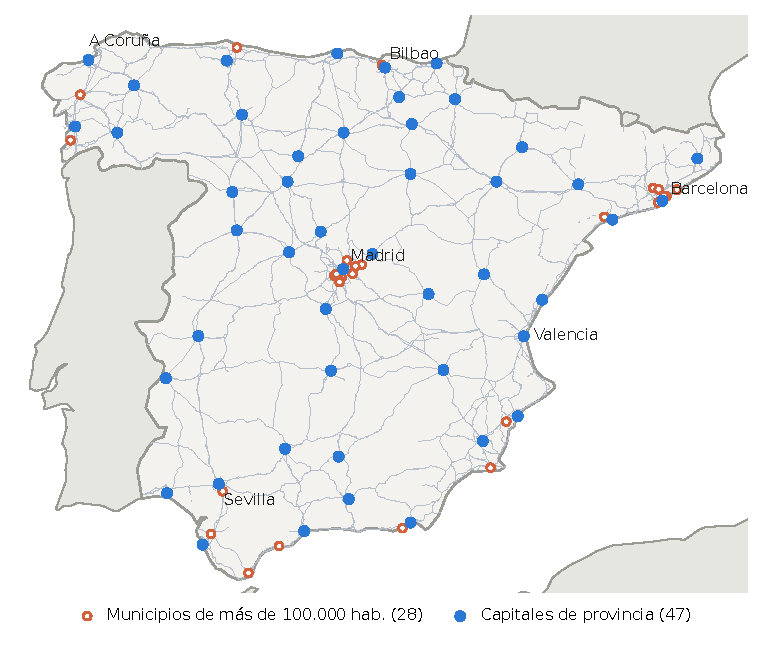
\includegraphics[width=0.78\linewidth]{red_ciudades.pdf}
  \caption{Las 75 ciudades del estudio sobre la red de autovías y vías rápidas (fondo gris). Los círculos azules son las 47 capitales de provincia; los círculos naranjas, los 28 municipios de más de 100.000 habitantes que no son capitales.}
  \label{fig:ciudades}
\end{figure}

\paragraph{Fuentes.} La lista de capitales y la población proceden del INE (\emph{Cifras oficiales de población de los municipios españoles: Revisión del Padrón Municipal}, datos a 1 de enero de 2025,
publicados el 11 de diciembre de 2025 en el BOE-A-2025-25362). La comunidad autónoma de cada ciudad se asignó con las tablas por provincia del INE. Las \textbf{coordenadas} proceden de los nodos
\texttt{place=city} o \texttt{place=town} de OpenStreetMap, el centro de cada núcleo urbano; no son una fuente oficial. Una primera geocodificación con Nominatim devolvía la provincia en lugar del
municipio para algunas capitales (Guadalajara, Palencia\dots) y el centro del término municipal en otras (Almería quedaba 14~km desplazada), por lo que se sustituyó por los nodos del propio extracto.

\section{De las ciudades a la red}

Cada ciudad se asocia al \emph{nodo de carretera más cercano}, mediante una búsqueda en un árbol $k$-d (\texttt{cKDTree} de SciPy) sobre coordenadas convertidas a kilómetros. Si ese nodo está a más de
$X=10$~km, la ciudad no está realmente conectada a esa versión de la red y se deja fuera de ella, registrando su distancia. Esto solo ocurre en una versión (sección~\ref{sec:redes}). La distancia entre la ciudad y su nodo
\emph{no} se suma a las distancias: es una simplificación del acceso que afecta por igual a todos los algoritmos.

\section{Tablas de distancias}

Para dos ciudades $a$ y $b$ con nodos asociados $u_a$ y $u_b$, la distancia entre ellas es la del camino mínimo en el grafo vial:
\begin{equation}\label{eq:dijkstra}
  D(a,b)\;=\;\min_{P:\,u_a\to u_b}\ \sum_{e\in P} w(e),
\end{equation}
donde $P$ recorre las aristas respetando los sentidos y $w$ es la longitud (\texttt{length}, que se convierte a kilómetros) o el tiempo de viaje (\texttt{travel\_time}). Se calcula con el algoritmo de Dijkstra~\cite{dijkstra1959} (implementación de SciPy) desde cada una de las 75 ciudades.
Como los sentidos únicos hacen que $D(a,b)\neq D(b,a)$, la tabla es asimétrica: por ejemplo, de Madrid a Sevilla hay 502~km y de Sevilla a Madrid, 517~km. Para el caso sin sentidos únicos se ignoran las direcciones y cada tramo cuesta lo
que la más barata de sus dos direcciones.

Los caminos mínimos cumplen la desigualdad triangular~\eqref{eq:triangular} por construcción, de modo que todas las versiones del problema son métricas (las no dirigidas, además, simétricas). Esto es lo que permite aplicar
Christofides con garantía a las versiones no dirigidas.

\section{Las versiones del problema}\label{sec:versiones}

Una \emph{versión} se define con cinco elecciones (tabla~\ref{tab:parametros}). Cada versión se carga con una función \texttt{cargar\_version(\dots)} que devuelve un grafo de NetworkX cuyos nodos son las ciudades y
cuyo peso \texttt{peso} es la distancia.

\begin{table}[htbp]
  \centering
  \caption{Parámetros que definen una versión del problema.}\label{tab:parametros}
  \small
  \begin{tabularx}{\linewidth}{@{}l X@{}}
    \toprule
    Parámetro & Valores \\
    \midrule
    \texttt{aristas} & \texttt{completo} (8 tipos de vía), \texttt{autovias\_principales} (sin secundarias), \texttt{solo\_autovias} y \texttt{sin\_autovias}. \\
    \texttt{nodos} & \texttt{capitales} (47 ciudades) o \texttt{capitales\_y\_100k} (75 ciudades). \\
    \texttt{ambito} & \texttt{espana} o una de las 15 comunidades autónomas peninsulares. \\
    \texttt{peso} & \texttt{km} (kilómetros) o \texttt{tiempo} (segundos, el registrado en el grafo). \\
    \texttt{general} & \texttt{multigrafo\_dirigido}, \texttt{grafo\_dirigido}, \texttt{multigrafo\_no\_dirigido} o \texttt{grafo\_simple\_no\_dirigido}. \\
    \bottomrule
  \end{tabularx}
\end{table}

\subsection{Cuántas versiones hay}

Combinando 4 redes, 2 pesos y dirigido o no dirigido se obtienen \textbf{16 tablas} de $75\times 75$ (en total, 0,9~MB). Cada versión es un \emph{trozo} de una de esas tablas, las filas y columnas
de las ciudades que correspondan. Guardar 480 grafos de carreteras ocuparía decenas de gigabytes; así, en cambio, quienes programan los algoritmos no necesitan el grafo grande.

El catálogo contiene \textbf{480 versiones}, que corresponden a \textbf{240 grafos de ciudades distintos}, porque entre dos nodos el camino mínimo solo usa la arista más barata, de modo que el multigrafo y el grafo simple
dan exactamente la misma tabla. De los 240 grafos, 32 son de toda España (44 a 75 ciudades) y 208 son regionales (4 a 13 ciudades). Las versiones regionales usan \emph{toda la red} (el mejor camino entre dos ciudades de una
comunidad puede salir de ella) y requieren un mínimo de $N_{\min}=4$ ciudades, lo que da 5 conjuntos de capitales (Andalucía, Castilla y León, Castilla-La Mancha, Cataluña y Galicia) y 8 de capitales más municipios de más de 100.000 habitantes
(los anteriores más Madrid, Comunidad Valenciana y País Vasco). Los tamaños regionales son 4, 5, 6, 8, 9, 11 y 13 ciudades, y son los que permiten aplicar los algoritmos exactos de enumeración a datos reales.

\subsection{Las cuatro versiones de carreteras}\label{sec:redes}

Las cuatro redes se obtienen filtrando aristas del grafo base y conservando, en cada caso, la mayor componente fuertemente conexa (tabla~\ref{tab:redes}).

\begin{table}[htbp]
  \centering
  \caption{Lo que queda en cada versión de carreteras.}\label{tab:redes}
  \small
  \begin{tabularx}{\linewidth}{@{}l r r r r X@{}}
    \toprule
    Red & Nodos & Aristas & Km & \makecell[r]{Nodos\\descartados} & Ciudades fuera \\
    \midrule
    \texttt{completo} & 179.594 & 309.250 & 182.760 & 0 & ninguna \\
    \texttt{autovias\_principales} & 115.476 & 190.221 & 111.121 & 5.885 & ninguna \\
    \texttt{solo\_autovias} & 19.239 & 24.450 & 28.921 & 14.027 & 3: Salamanca (62,7~km), Badajoz (50,5~km), Cuenca (39,6~km) \\
    \texttt{sin\_autovias} & 146.903 & 256.301 & 140.040 & 8.464 & ninguna \\
    \bottomrule
  \end{tabularx}
\end{table}

\texttt{autovias\_principales} elimina las carreteras secundarias; \texttt{solo\_autovias} deja únicamente autopistas y autovías; \texttt{sin\_autovias} excluye autopistas y autovías (la red «para ir por carreteras convencionales»).
En \texttt{solo\_autovias}, tres ciudades quedan a más de 10~km de la red y se dejan fuera, de modo que esa versión tiene 44 o 72 ciudades en lugar de 47 o 75.

\section{Decisiones de diseño}

\begin{itemize}
  \item \textbf{Bicicleta y a pie no son versiones aparte.} Con velocidad constante, el tiempo es proporcional a la distancia, así que el camino más corto y el recorrido óptimo coinciden con los de kilómetros.
        El caso «a pie o en bici» es \texttt{sin\_autovias} en kilómetros; para horas basta dividir (entre 20 en bicicleta, entre 5 a pie). Descartamos esas versiones para no duplicar resultados idénticos.
  \item \textbf{Las ciudades fuera de la red no se «arreglan».} Como ocurre con las islas, el viajante no puede visitar una ciudad desconectada; se registra y se deja fuera. Por eso Castilla y León pasa de 9 a 8 capitales en \texttt{solo\_autovias}.
  \item \textbf{Modelo no dirigido.} Al ignorar los sentidos únicos, cada tramo vale lo que la más barata de sus dos direcciones. Un atajo por una rampa en contradirección es un efecto pequeño, pero existe.
  \item \textbf{Una sola red maestra.} Todo se deriva del grafo base; así cualquier cambio en los criterios (por ejemplo, el umbral de 10~km) se propaga recalculando las 16 tablas, unos dos minutos.
\end{itemize}

\section{Comprobaciones}

Sobre las 16 tablas se comprueba que las distancias son finitas y no negativas, que la diagonal es cero, que las tablas no dirigidas son simétricas, que la distancia no dirigida nunca supera a la dirigida y que se cumple la
desigualdad triangular (con una tolerancia de 0,01 por el redondeo a tres decimales al guardar). Además, se cargaron sin error las 480 versiones del catálogo.

\chapter{Los algoritmos}\label{cap:algoritmos}

\section{Criterios de elección}

Hemos implementado ocho algoritmos de modo que estén representadas las familias clásicas de métodos para el TSP, con cuya comparación se puede responder a las preguntas del estudio:

\begin{itemize}
  \item \textbf{Exactos} (garantizan el óptimo): \emph{fuerza bruta}, que enumera todas las rutas; \emph{Held--Karp}, que reduce la enumeración con programación dinámica; y \emph{DFJ}, que usa programación entera con restricciones de subciclo.
        Cubren tres estrategias muy distintas para llegar al mismo resultado.
  \item \textbf{Heurísticos y aproximados}: el \emph{vecino más cercano} (constructivo, el más simple), el \emph{2-opt} (mejora local sobre una ruta existente) y \emph{Christofides} (aproximación con garantía demostrada).
  \item \textbf{Metaheurísticas}, que exploran el espacio de soluciones con azar: el \emph{recocido simulado} (inspirado en la física) y el \emph{algoritmo genético} (inspirado en la evolución).
\end{itemize}

Quedó fuera de la lista el algoritmo de Dijkstra, que a veces se cita en este contexto pero no resuelve el viajante: calcula el camino más corto \emph{entre dos puntos}, no un recorrido que pase por todos. En este trabajo se usa
precisamente para construir las tablas de distancias entre ciudades (capítulo~\ref{cap:versiones}). Tampoco se incluye un «algoritmo hamiltoniano» aparte, porque el TSP es, precisamente, encontrar el ciclo hamiltoniano de menor coste.

\section{Notación y contrato común}

Todos los algoritmos reciben el grafo de ciudades $K$, completo, donde $K[a][b]$ es el coste $c(a,b)$ de ir de $a$ a $b$, y una ciudad de partida opcional. Devuelven una ruta (lista con todas las ciudades, cada una una vez,
en el orden en que se visitan) y su coste $C(\pi)$ según la ecuación~\eqref{eq:coste}, que incluye la vuelta. Esta interfaz común es lo que permite comparar los algoritmos con una misma batería de pruebas. Todos funcionan con grafos dirigidos
(asimétricos) y no dirigidos, salvo Christofides, que necesita simetría.

La tabla~\ref{tab:fichas} resume las propiedades de los ocho algoritmos. En las secciones siguientes se explica cada uno: la idea, el pseudocódigo, la complejidad en notación $O$ y sus propiedades. Las complejidades se expresan en
función del número de ciudades $n$.

\begin{table}[htbp]
  \centering
  \caption{Resumen de los ocho algoritmos. $G$ = generaciones, $P$ = población, $q$ = intentos de mutación.}\label{tab:fichas}
  \footnotesize
  \begin{tabularx}{\linewidth}{@{}l l l X X@{}}
    \toprule
    Algoritmo & Autor & Tipo & Tiempo & Memoria \\
    \midrule
    Fuerza bruta & Pablo & exacto & $O((n-1)!\cdot n)$ & $O(n)$ \\
    Held--Karp & Raimundo & exacto (prog. dinámica) & $O(n^2\cdot 2^n)$ & $O(n\cdot 2^n)$ \\
    DFJ & Jiahao & exacto (prog. entera) & $O(2^n)$ en el peor caso & $O(n^2)$ en la práctica \\
    Vecino más cercano & Pablo & heurístico voraz & $O(n^2)$ & $O(n)$ \\
    2-opt & Raimundo & mejora local & $O(n^2)$ por vuelta & $O(n^2)$ \\
    Christofides & Raimundo & aproximado (1,5) & $O(n^3)$ & $O(n^2)$ \\
    Recocido simulado & Juan & metaheurística & niveles de temperatura $\times$ iteraciones & $O(n^2)$ \\
    Genético & Raimundo & metaheurística & $O(G\cdot P\cdot n\cdot q)$ & $O(P\cdot n)$ \\
    \bottomrule
  \end{tabularx}
\end{table}

\section{Fuerza bruta}\label{sec:fuerzabruta}

\textbf{Idea.} Probar todas las rutas posibles y quedarse con la más corta. Como cualquier ciclo se puede escribir empezando por la ciudad de partida, hay $(n-1)!$ rutas distintas que hay que evaluar; cada una cuesta $O(n)$ sumar,
de ahí la complejidad $O((n-1)!\cdot n)$. La memoria es $O(n)$ porque solo se guardan la mejor ruta y la permutación en curso.

\begin{algorithm}[htbp]
  \caption{Fuerza bruta}\label{alg:fb}
  \begin{algorithmic}[1]
    \Require grafo $K$ con $n$ ciudades, ciudad de partida $s$
    \Ensure ruta óptima y su coste
    \State $mejor \gets \infty$
    \ForAll{ordenación $\sigma$ de las $n-1$ ciudades distintas de $s$}
      \State $ruta \gets [s]+\sigma$ \;;\; $coste \gets C(ruta)$ \Comentario{incluye la vuelta}
      \If{$coste < mejor$} \State $mejor \gets coste$ \;;\; guardar $ruta$ \EndIf
    \EndFor
    \State \Return mejor ruta
  \end{algorithmic}
\end{algorithm}

\textbf{Propiedades.} Exacto y determinista; no necesita distancias simétricas. Su problema es el tiempo: 10 ciudades se resuelven en medio segundo, 11 en unos 20 segundos y cada ciudad más multiplica el tiempo por $n$, de modo que con 13 serían
del orden de 50 minutos. Es útil como referencia exacta para instancias muy pequeñas.

\section{Held--Karp (programación dinámica)}\label{sec:heldkarp}

\textbf{Idea.} Muchas de las $(n-1)!$ rutas comparten tramos: si dos rutas empiezan en la ciudad de partida, pasan por las mismas ciudades (en distinto orden) y terminan en la misma, solo importa cuál de los dos tramos es más
corto. Held y Karp~\cite{heldkarp1962} (y, de forma independiente, Bellman~\cite{bellman1962}) aprovecharon esa observación con \emph{programación dinámica}: se resuelve cada subproblema una sola vez y se reutiliza.

Se fija una ciudad de partida $0$. Para cada subconjunto $S$ de las demás ciudades y cada $j\in S$, sea $d[S][j]$ el coste del camino más corto que sale de $0$, visita exactamente las ciudades de $S$ y termina en $j$. Entonces
\begin{equation}\label{eq:heldkarp}
  d[S][j]\;=\;\min_{i\in S\setminus\{j\}}\Bigl(d\bigl[S\setminus\{j\}\bigr][i]+c(i,j)\Bigr),\qquad d[\{j\}][j]=c(0,j),
\end{equation}
y el coste óptimo es $\min_{j}\bigl(d[V\setminus\{0\}][j]+c(j,0)\bigr)$. La ruta se reconstruye hacia atrás, recordando para cada estado el $i$ que dio el mínimo.

\begin{algorithm}[htbp]
  \caption{Held--Karp}\label{alg:hk}
  \begin{algorithmic}[1]
    \Require grafo $K$, ciudad de partida $0$
    \Ensure ruta óptima y su coste
    \State $d[\{j\}][j] \gets c(0,j)$ para cada ciudad $j\neq 0$
    \For{$k \gets 2$ \textbf{hasta} $n-1$} \Comentario{tamaño del subconjunto}
      \ForAll{subconjunto $S$ de tamaño $k$ y cada $j\in S$}
        \State $d[S][j] \gets \min_{i\in S\setminus\{j\}}\bigl(d[S\setminus\{j\}][i]+c(i,j)\bigr)$
      \EndFor
    \EndFor
    \State $j^{*} \gets \arg\min_j\bigl(d[V\setminus\{0\}][j]+c(j,0)\bigr)$
    \State \Return ruta reconstruida hacia atrás desde $j^{*}$
  \end{algorithmic}
\end{algorithm}

\textbf{Complejidad.} Hay $2^{n-1}(n-1)$ estados y cada uno se calcula probando hasta $n-1$ ciudades anteriores, luego el \textbf{tiempo} es $O(n^2\cdot 2^n)$, frente al $O((n-1)!)$ de la fuerza bruta. La \textbf{memoria} es $O(n\cdot 2^n)$:
la tabla $d$ ocupa $8\,(n-1)\,2^{n-1}$ bytes (unos 80~MB con 20 ciudades, 170~MB con 21 y más de 700~MB con 22). Es el verdadero límite de este algoritmo, y por eso la implementación se niega a trabajar con más de 21 ciudades.

\textbf{Implementación.} Cada subconjunto se guarda como un entero (una máscara de bits) y los subconjuntos de cada tamaño se procesan a la vez con NumPy. \textbf{Propiedades:} exacto, determinista, sirve para el caso dirigido y el no dirigido.

\section{DFJ: programación entera con restricciones de subciclo}\label{sec:dfj}

\textbf{Idea.} La formulación de Dantzig, Fulkerson y Johnson~\cite{dfj1954} plantea el TSP como un problema de programación entera con una variable binaria $x_{ij}$ por arista dirigida (vale $1$ si el viajante va de $i$ a $j$):
\begin{equation}\label{eq:dfj}
\begin{aligned}
  \min\ & \sum_{i\neq j} c(i,j)\,x_{ij}\\
  \text{s.a. } & \sum_{j\neq i} x_{ij}=1\quad\forall i,\qquad \sum_{i\neq j} x_{ij}=1\quad\forall j,\qquad x_{ij}\in\{0,1\}.
\end{aligned}
\end{equation}
Las dos primeras familias de restricciones (una salida y una entrada por ciudad) definen el \emph{problema de asignación}, que es más fácil que el TSP pero admite soluciones formadas por \emph{varios circuitos sueltos} (subciclos) en lugar de un único ciclo.
Para evitarlo se añade, para cada subconjunto $S$ de ciudades que forma un subciclo, una restricción de conectividad
\begin{equation}\label{eq:subciclo}
  \sum_{i\in S}\ \sum_{j\notin S} x_{ij}\;\ge\;1,
\end{equation}
que obliga a que al menos una arista salga del grupo. Como hay un número exponencial de subconjuntos, las restricciones no se añaden todas desde el principio: se resuelve el modelo, se detectan los subciclos de la solución, se añaden sus restricciones
y se vuelve a resolver, hasta que la solución sea un único ciclo.

\begin{algorithm}[htbp]
  \caption{DFJ con eliminación iterativa de subciclos}\label{alg:dfj}
  \begin{algorithmic}[1]
    \Require grafo $K$
    \Ensure ruta óptima y su coste
    \State modelo $\gets$ problema de asignación~\eqref{eq:dfj}
    \Repeat
      \State $x^{*} \gets$ resolver el modelo entero con un \emph{solver}
      \State $\mathcal{C} \gets$ componentes (circuitos) de la solución $x^{*}$
      \If{$|\mathcal{C}|>1$}
        \ForAll{circuito $S\in\mathcal{C}$} \State añadir al modelo la restricción~\eqref{eq:subciclo} \EndFor
      \EndIf
    \Until{$|\mathcal{C}|=1$}
    \State \Return el ciclo $x^{*}$
  \end{algorithmic}
\end{algorithm}

\textbf{Complejidad y propiedades.} En el peor caso el tiempo es exponencial, porque resolver cada modelo es NP-difícil y el número de restricciones puede crecer exponencialmente. En la práctica, con los \emph{solvers} modernos, suele bastar con muy pocas iteraciones
(en nuestras instancias, entre 2 y 10), y la memoria es del orden de $O(n^2)$ por las variables del modelo. Es exacto, determinista y válido para grafos dirigidos y no dirigidos (en este último caso se convierte el grafo a dirigido, con una arista por sentido y el mismo peso).
Usamos PuLP con el \emph{solver} CBC. En el capítulo~\ref{cap:resultados} se verá que este algoritmo resuelve las 75 ciudades al óptimo en unos 4~segundos, muy por encima del límite de los exactos de enumeración.

\section{Vecino más cercano}\label{sec:vecino}

\textbf{Idea.} Es la ruta del viajante que no planifica: en cada ciudad, ir a la más cercana que todavía no se haya visitado. Es un algoritmo \emph{voraz}: toma siempre la mejor opción local sin mirar atrás. A cambio de su simplicidad renuncia a la optimalidad: una elección buena ahora
puede dejar aislada una ciudad lejana y encarecer el final del recorrido.

\begin{algorithm}[htbp]
  \caption{Vecino más cercano}\label{alg:nn}
  \begin{algorithmic}[1]
    \Require grafo $K$, ciudad de partida $s$
    \Ensure ruta y su coste
    \State $ruta \gets [s]$ \;;\; $pendientes \gets V\setminus\{s\}$
    \While{$pendientes\neq\emptyset$}
      \State $a \gets$ última ciudad de $ruta$
      \State $b \gets \arg\min_{x\in pendientes} c(a,x)$ \Comentario{la más cercana}
      \State añadir $b$ a $ruta$ \;;\; quitar $b$ de $pendientes$
    \EndWhile
    \State \Return $ruta$, $C(ruta)$ \Comentario{la vuelta cierra el ciclo}
  \end{algorithmic}
\end{algorithm}

\textbf{Complejidad y propiedades.} Hay $n-1$ pasos y en cada uno se comparan hasta $n-1$ ciudades, luego $O(n^2)$ en tiempo y $O(n)$ en memoria adicional. Es determinista (los empates se resuelven por orden alfabético), no necesita simetría y
no ofrece ninguna garantía de calidad: incluso con distancias métricas, el peor caso puede ser $\Theta(\log n)$ veces el óptimo. Depende de la ciudad de partida. Se usa aquí como solución inicial de otras técnicas (2-opt) y como línea base.

\section{2-opt}\label{sec:dosopt}

\textbf{Idea.} Es una \emph{búsqueda local}~\cite{croes1958}: parte de una ruta cualquiera y la mejora con pequeños cambios mientras sea posible. El cambio de 2-opt es el que haría una persona mirando el mapa: si dos tramos de la ruta se cruzan,
se deshacen y se vuelven a unir al revés, lo que elimina el cruce y casi siempre acorta el camino.

Concretamente, se toman dos aristas $(a\to b)$ y $(c\to d)$ de la ruta (con $b$ justo después de $a$ y $d$ justo después de $c$) y se sustituyen por $(a\to c)$ y $(b\to d)$, invirtiendo el tramo que queda entre medias. El cambio mejora la ruta si
\begin{equation}\label{eq:dosopt}
  \Delta\;=\;c(a,c)+c(b,d)-c(a,b)-c(c,d)\;<\;0,
\end{equation}
donde, en un grafo \emph{dirigido}, hay que sumar además la diferencia entre recorrer el tramo invertido al revés y hacia delante (porque ir de $x$ a $y$ no cuesta lo mismo que de $y$ a $x$); la implementación lo calcula en tiempo constante con sumas acumuladas
y vale igual para el caso no dirigido, donde esa diferencia es cero.

\begin{algorithm}[htbp]
  \caption{2-opt}\label{alg:2opt}
  \begin{algorithmic}[1]
    \Require grafo $K$, ciudad de partida $s$
    \Ensure ruta (óptimo local) y su coste
    \State $ruta \gets$ ruta del vecino más cercano desde $s$
    \Repeat
      \ForAll{par de tramos $(a\to b)$, $(c\to d)$ no contiguos de $ruta$}
        \State calcular $\Delta$ \Comentario{ecuación~\eqref{eq:dosopt}}
      \EndFor
      \State $(a,b,c,d)\gets$ el par con menor $\Delta$
      \If{$\Delta<0$} \State invertir el tramo de $b$ a $c$ en $ruta$ \EndIf
    \Until{ningún cambio mejora la ruta}
    \State \Return $ruta$
  \end{algorithmic}
\end{algorithm}

\textbf{Complejidad y propiedades.} Cada vuelta evalúa todos los pares de tramos (con \texttt{numpy}, en forma de matrices $n\times n$), luego cuesta $O(n^2)$ en tiempo y memoria; el número de vueltas es del orden de $n$ en la práctica, así que el total ronda $O(n^3)$,
aunque no hay una cota polinómica en el peor caso. Es una heurística: se detiene en el primer \emph{óptimo local}, que puede no ser el óptimo global; sin garantía de calidad útil, pero en la práctica queda a pocos puntos porcentuales del óptimo.
Es determinista dada la ruta de partida y funciona con grafos dirigidos y no dirigidos.

\section{Christofides}\label{sec:christofides}

\textbf{Idea.} Es el algoritmo de aproximación con garantía más conocido para el TSP métrico: la ruta que devuelve nunca cuesta más de $1{,}5$ veces el óptimo~\cite{christofides1976}. Se construye en cinco pasos:
\begin{enumerate}[label=\arabic*.]
  \item \textbf{Árbol de expansión mínimo} (\emph{MST}): une todas las ciudades con el menor coste total y sin ciclos. Su coste es una cota inferior del óptimo: si a un ciclo óptimo se le quita una arista queda un árbol, y no puede costar menos que el mínimo.
  \item Se identifican las ciudades de \textbf{grado impar} en el árbol (siempre hay un número par de ellas).
  \item \textbf{Emparejamiento perfecto de coste mínimo} entre ellas, que se calcula con el algoritmo de Edmonds~\cite{edmonds1965} (\emph{blossom}). Su coste es, como mucho, la mitad del óptimo.
  \item Árbol y emparejamiento forman un multigrafo en el que todas las ciudades tienen grado par, de modo que existe un \textbf{circuito euleriano}, que recorre cada arista una vez.
  \item \textbf{Atajos}: se recorre el circuito saltándose las ciudades ya visitadas. Por la desigualdad triangular~\eqref{eq:triangular}, ir directo nunca cuesta más que dar el rodeo.
\end{enumerate}
La garantía sale de sumar: $C \le c(\text{MST}) + c(\text{emparejamiento}) \le C^{*} + \tfrac12 C^{*} = 1{,}5\,C^{*}$.

\begin{algorithm}[htbp]
  \caption{Christofides (grafo no dirigido)}\label{alg:chr}
  \begin{algorithmic}[1]
    \Require grafo no dirigido $K$ con distancias métricas
    \Ensure ruta con coste $\le 1{,}5\,C^{*}$
    \State $T \gets$ árbol de expansión mínimo de $K$
    \State $I \gets$ ciudades de grado impar en $T$
    \State $M \gets$ emparejamiento perfecto de coste mínimo entre las ciudades de $I$
    \State $circuito \gets$ circuito euleriano del multigrafo $T\cup M$
    \State $ruta \gets$ $circuito$ sin repetir ciudades (se salta cada ciudad ya visitada)
    \State \Return $ruta$
  \end{algorithmic}
\end{algorithm}

\textbf{Complejidad y propiedades.} El árbol cuesta $O(n^2\log n)$, el emparejamiento \emph{blossom} sobre las ciudades impares $O(n^3)$ en el peor caso y el circuito euleriano $O(n)$; domina el emparejamiento, luego $O(n^3)$ en tiempo y $O(n^2)$ en memoria.
\textbf{Necesita un grafo no dirigido} (distancias simétricas) y métrico, condiciones que cumplen las versiones no dirigidas de este trabajo. La implementación rechaza grafos dirigidos con un error explícito. Es determinista en lo que depende de los datos.

\section{Recocido simulado}\label{sec:recocido}

\textbf{Idea.} El recocido simulado~\cite{kirkpatrick1983} es una metaheurística inspirada en el proceso metalúrgico de recocido. Una búsqueda local como el 2-opt se detiene en el primer valle (óptimo local) porque cualquier cambio inmediato
empeora la ruta. El recocido supera esta barrera aceptando también, con cierta probabilidad, cambios que \emph{empeoran} la ruta. Esa probabilidad depende de una \emph{temperatura} $T$ que va bajando poco a poco: a temperaturas altas se acepta casi todo y se explora; al enfriarse,
el sistema se vuelve cada vez más voraz y se asienta en un buen valle. Matemáticamente es el algoritmo de Metropolis--Hastings~\cite{metropolis1953} orientado a la optimización: un cambio que aumenta el coste en $\Delta F>0$ se acepta con probabilidad
\begin{equation}\label{eq:metropolis}
  P\;=\;e^{-\Delta F/T}.
\end{equation}

\begin{algorithm}[htbp]
  \caption{Recocido simulado}\label{alg:sa}
  \begin{algorithmic}[1]
    \Require grafo $K$, factor de enfriamiento $\alpha=0{,}95$, temperatura mínima $T_{\min}$
    \Ensure ruta y su coste
    \State $ruta \gets$ ruta al azar \;;\; $mejor \gets ruta$ \;;\; $T \gets 0{,}15\cdot C(ruta)$
    \While{$T > T_{\min}$}
      \State repetir $n_{\text{iter}}$ veces:
      \State \hspace{1.2em} proponer invertir un tramo al azar (cambio 2-opt) y calcular $\Delta F$
      \State \hspace{1.2em} \textbf{si} $\Delta F\le 0$ \textbf{o} $\text{azar}(0,1)<e^{-\Delta F/T}$ \textbf{entonces} aceptar el cambio
      \State \hspace{1.2em} actualizar $mejor$ si la ruta mejora
      \State $T \gets \alpha\cdot T$ \Comentario{enfriar}
    \EndWhile
    \State \Return $mejor$
  \end{algorithmic}
\end{algorithm}

\textbf{Complejidad y propiedades.} Es una metaheurística estocástica: no garantiza el óptimo ni ofrece una cota de calidad, y el resultado depende del azar (por eso se mide con varias semillas). Evaluar el efecto de un cambio de 2-opt cuesta $O(1)$ (solo cambian cuatro aristas), pero aceptar el cambio
obliga a actualizar la ruta en $O(n)$; el número de iteraciones por nivel de temperatura crece con $n$. Funciona con grafos dirigidos y no dirigidos. Su implementación es obra de Juan, que además calcula una cota inferior del óptimo con un 1-árbol para acotar el error de cada ejecución.

\section{Algoritmo genético}\label{sec:genetico}

\textbf{Idea.} Los algoritmos genéticos~\cite{holland1975} imitan la evolución de las especies: se mantiene una \emph{población} de rutas que evoluciona durante muchas \emph{generaciones}; las rutas más cortas tienen más probabilidad de reproducirse, sus «hijos» combinan características de los padres
y, de vez en cuando, sufren pequeñas \emph{mutaciones}. Los elementos son:
\begin{itemize}
  \item \textbf{Individuo:} una ruta, es decir, una permutación de las ciudades (la de partida va fija en primer lugar). Siempre es válida.
  \item \textbf{Aptitud:} el coste del ciclo; cuanto menor, mejor.
  \item \textbf{Selección por torneo:} cada padre es el mejor de 3 individuos elegidos al azar.
  \item \textbf{Cruce por orden (OX)}~\cite{davis1985}: el hijo hereda de un padre un tramo seguido y el resto de ciudades en el orden en que aparecen en el otro padre, así nunca repite ni omite ninguna.
  \item \textbf{Mutación guiada:} con probabilidad $p_m$ se prueban $q=10$ inversiones de tramo al azar (el movimiento del 2-opt) y el individuo se queda con la mejor, \emph{solo si mejora} su coste.
  \item \textbf{Elitismo:} las 2 mejores rutas pasan intactas a la siguiente generación.
\end{itemize}

\begin{algorithm}[htbp]
  \caption{Algoritmo genético}\label{alg:gen}
  \begin{algorithmic}[1]
    \Require grafo $K$, población $P=150$, generaciones máximas $G=500$, probabilidad de mutación $p_m=0{,}5$
    \Ensure ruta y su coste
    \State $poblacion \gets$ $P$ rutas aleatorias
    \Repeat
      \State $nueva \gets$ las 2 mejores rutas de $poblacion$
      \While{$|nueva| < P$}
        \State $p_1,p_2 \gets$ dos padres por torneo (el mejor de 3 al azar)
        \State $hijo \gets$ \textsc{CruceOX}$(p_1,p_2)$
        \State con probabilidad $p_m$, \textsc{MutaciónGuiada}$(hijo)$
        \State añadir $hijo$ a $nueva$
      \EndWhile
      \State $poblacion \gets nueva$ \;;\; actualizar la mejor ruta
    \Until{$G$ generaciones o 150 sin mejorar}
    \State \Return mejor ruta
  \end{algorithmic}
\end{algorithm}

\textbf{Complejidad y propiedades.} Cada generación cruza y evalúa $P$ rutas de longitud $n$ (y la mutación prueba $q$ variantes), así que el tiempo es $O(G\cdot P\cdot n\cdot q)$, \emph{lineal en $n$} por generación, y la memoria $O(P\cdot n)$.
Es estocástico, pero reproducible fijando la semilla, y no tiene garantía de calidad. Una lección del desarrollo merece señalarse: la primera versión, con mutaciones aleatorias simples, quedaba entre un 19~\% y un 37~\% por encima del óptimo con 47 ciudades;
la mutación guiada (que incorpora una pequeña búsqueda local) lo redujo a un 2--5~\%.

\section{Quién hizo qué}

Cuatro personas implementaron los ocho algoritmos. Pablo programó la fuerza bruta y el vecino más cercano, Jiahao programó DFJ, Juan programó el recocido simulado y Raimundo programó Held--Karp, 2-opt, Christofides y el genético. Cada algoritmo vive en su propio \emph{notebook}
con la misma estructura (ficha, teoría, código, pruebas y resultados), que una herramienta integra después en el \emph{notebook} principal. El capítulo~\ref{cap:organizacion} describe este flujo de trabajo.

\chapter{Metodología experimental}\label{cap:metodologia}

Este capítulo describe cómo se diseñó y se ejecutó el estudio empírico: qué se mide, sobre qué instancias, con qué reglas de aplicabilidad y con qué precauciones para que los resultados sean fiables y reproducibles.

\section{Qué se mide}

Para cada ejecución de un algoritmo sobre una instancia se registran cuatro magnitudes:
\begin{itemize}
  \item el \textbf{coste} $C$ de la ruta devuelta (en kilómetros o en horas, según la versión);
  \item el \textbf{tiempo} de cálculo, medido con \texttt{perf\_counter};
  \item el \textbf{pico de memoria} reservada por Python, medido con \texttt{tracemalloc}; y
  \item la \textbf{desviación respecto al óptimo}, definida para cada instancia como
  \begin{equation}\label{eq:desviacion}
    \delta\;=\;\frac{C-C^{*}}{C^{*}}\times 100\ \%,
  \end{equation}
  donde $C^{*}$ es el coste óptimo de esa instancia.
\end{itemize}
El óptimo $C^{*}$ de cada instancia es el coste que devuelve \textbf{DFJ}, un algoritmo exacto que se ejecuta en todas las versiones. Para comprobar que esta referencia es fiable, el estudio verifica que
\emph{los tres algoritmos exactos coinciden} siempre que se pueden comparar (sección~\ref{sec:validacion}). Un caso aparte es la memoria de DFJ, de la que solo se cuenta la reservada por Python; la del \emph{solver} CBC, que corre como proceso aparte, no se mide.

\section{Instancias: dos estudios complementarios}

El estudio se divide en dos partes que responden a preguntas distintas:
\begin{description}[leftmargin=0pt,labelindent=0pt,style=nextline]
  \item[Estudio A: versiones reales.] Los \textbf{240 grafos de ciudades distintos} del catálogo (capítulo~\ref{cap:versiones}): 4 redes, 2 conjuntos de ciudades, 16 ámbitos geográficos, 2 pesos y dirigido o no dirigido.
        De ellos, 32 son de toda España (44 a 75 ciudades) y 208 son regionales (4 a 13 ciudades). Sirve para ver cómo cambian los resultados con la red, el peso y el sentido de las vías.
  \item[Estudio B: curva de escalado.] Subconjuntos \textbf{aleatorios} de las 75 ciudades, de $n=5,6,\dots,12,14,16,18,20,25,30,40,47,60$ y $75$ ciudades, con tres subconjuntos distintos por tamaño (uno solo para $n=75$, que es el conjunto completo),
        sobre la versión \texttt{completo}/km, dirigida y no dirigida. Los subconjuntos se generan con semilla fija, de modo que son reproducibles. Sirve para ajustar cómo crecen el tiempo y la memoria con $n$.
\end{description}

\section{Qué algoritmo se puede aplicar a qué versión}\label{sec:aplicabilidad}

No todos los algoritmos se pueden ejecutar sobre todas las versiones, y esa limitación es un resultado en sí misma. Se aplican tres reglas, que el programa del estudio registra junto con su motivo (tabla~\ref{tab:aplicabilidad}):
\begin{itemize}
  \item \textbf{Fuerza bruta:} solo con $n\le 11$ ciudades. Hay $(n-1)!$ rutas: con 11 ciudades son 3,6 millones y tarda unos segundos; con 12, más de un minuto, y con 13, del orden de media hora.
  \item \textbf{Held--Karp:} solo con $n\le 21$ ciudades, porque su tabla ocupa $8\,(n-1)\,2^{n-1}$ bytes: 170~MB con 21 ciudades y más de 700~MB con 22.
  \item \textbf{Christofides:} solo en grafos \emph{no dirigidos}, porque necesita distancias simétricas.
\end{itemize}

\begin{table}[htbp]
  \centering
  \caption{Aplicabilidad de cada algoritmo sobre los 240 grafos del estudio A.}\label{tab:aplicabilidad}
  \small
  \begin{tabularx}{\linewidth}{@{}l r X@{}}
    \toprule
    Algoritmo & Versiones & Motivo de la exclusión \\
    \midrule
    Fuerza bruta & 192 & más de 11 ciudades (las 32 de toda España y las 16 de Andalucía, con 13 ciudades) \\
    Held--Karp & 208 & más de 21 ciudades (las 32 de toda España) \\
    Christofides & 120 & necesita un grafo no dirigido: se excluyen las 120 versiones dirigidas \\
    DFJ, vecino más cercano, 2-opt, recocido, genético & 240 & ninguna \\
    \bottomrule
  \end{tabularx}
\end{table}

Una consecuencia importante: en las 32 versiones de toda España (44 a 75 ciudades), \textbf{DFJ es el único algoritmo exacto aplicable}; los exactos de enumeración solo se pueden usar en las versiones regionales y en el estudio B hasta 11 y 20 ciudades.

\section{Medir el tiempo: paralelo y en serie}\label{sec:paralelo}

El estudio completo supone miles de ejecuciones, que se reparten entre varios procesos. Pero el coste de una ruta no depende de la carga del ordenador y el tiempo sí: con varios procesos a la vez se comparten núcleos físicos, memoria caché y reloj.
El equipo usado es un portátil con un procesador de cuatro núcleos físicos (ocho hilos) y frecuencia sostenida baja, y comprobamos que con seis procesos en paralelo la fuerza bruta de 11 ciudades pasa de unos 6~s a más de 40~s.
Por eso el estudio se hace en \textbf{dos pasadas}:
\begin{enumerate}
  \item \textbf{En paralelo} (seis procesos, 4.470 ejecuciones, unos 42 minutos): se usa para los \emph{costes} y las comparaciones de calidad, que no dependen de la carga.
  \item \textbf{En serie} (un solo proceso, 236 ejecuciones, unos 15 minutos): repite el estudio B con una instancia y una semilla por tamaño, con el equipo en reposo, y se usa para los \emph{tiempos y la memoria}.
\end{enumerate}
Una \textbf{calibración} repite en serie 15 tareas de la pasada en paralelo y mide cuánto las distorsiona (sección~\ref{sec:calibracion}).

\section{Algoritmos con azar y otros controles}

\begin{itemize}
  \item \textbf{Semillas.} El genético se ejecuta con 3 semillas y el recocido con 5; los resultados de estos dos algoritmos se resumen con medias y dispersión.
  \item \textbf{Ciudad de partida.} Es siempre Madrid (o la primera ciudad si Madrid no está en la instancia), para que las filas sean comparables. El vecino más cercano depende de ella; el resto no cambia el óptimo.
  \item \textbf{Ruido en tiempos pequeños.} Si una ejecución determinista dura menos de 50~ms, se repite cuatro veces más y se toma el mínimo.
  \item \textbf{Parada de seguridad.} Si pasan 15 minutos sin ningún resultado nuevo, el programa se detiene, y se puede reanudar sin perder lo hecho porque cada resultado se guarda al llegar.
  \item \textbf{Código real.} Los algoritmos no se copian en el programa del estudio: se extrae el código de sus \emph{notebooks}, de modo que lo que se mide es exactamente lo que se explica en el trabajo.
\end{itemize}

\section{Validación cruzada y control de calidad}\label{sec:validacion}

Además de medir, el estudio contrasta los algoritmos entre sí. En cada instancia se comprueba que: (i)~fuerza bruta, Held--Karp y DFJ devuelven el mismo coste (tolerancia del 0,1~\%, la del \emph{solver});
(ii)~ninguna heurística devuelve un coste inferior al óptimo, lo que delataría un error; y (iii)~cada ruta es válida (visita cada ciudad una vez) y su coste coincide con el recalculado.

Este control resultó decisivo: al ejecutar por primera vez los algoritmos sobre grafos \emph{no dirigidos}, el recocido simulado entró en un bucle infinito y el modelo de DFJ se planteaba mal; ambos fallos se debían a cómo trataban las aristas de un grafo no dirigido
y no se habían detectado en las pruebas individuales, hechas solo con grafos dirigidos. Se corrigieron con pocas líneas y se documentaron (sección~\ref{sec:problemas}).

\section{Amenazas a la validez}

\begin{itemize}
  \item \textbf{Tamaño de las instancias.} El máximo son 75 ciudades; con muchas más, DFJ dejaría de ser inmediato y los metaheurísticos podrían ganar terreno. No se ha medido.
  \item \textbf{Un solo subconjunto con $n=75$.} Es el conjunto completo; los tamaños menores usan tres subconjuntos distintos.
  \item \textbf{Parámetros por defecto.} Los metaheurísticos no se ajustaron a cada tamaño; con otros parámetros los resultados podrían cambiar.
  \item \textbf{Memoria incompleta en DFJ.} Solo se contabiliza la memoria reservada por Python, no la del \emph{solver}.
  \item \textbf{Un único equipo.} Los tiempos absolutos dependen del ordenador; lo que importa son las proporciones y el crecimiento.
\end{itemize}

\chapter{Resultados}\label{cap:resultados}

Se presentan los resultados del estudio empírico (4.470 ejecuciones en paralelo y 236 en serie, sin ningún fallo), siguiendo las cinco preguntas del capítulo~\ref{cap:intro}. Los tiempos absolutos dependen del equipo; interesan sobre todo
las proporciones y el crecimiento con el número de ciudades.

\section{Validación: los algoritmos exactos coinciden}

Fuerza bruta, Held--Karp y DFJ dan exactamente el mismo coste en todas las instancias en las que se pueden comparar: \textbf{234 instancias} (fuerza bruta frente a DFJ) y \textbf{280} (Held--Karp frente a DFJ), con cero discrepancias. Ninguna heurística devuelve un coste
inferior al óptimo. Este resultado respalda tanto la corrección de las tres implementaciones, que son muy distintas entre sí (enumeración, programación dinámica y programación entera), como el uso de DFJ como referencia del óptimo.

\section{Complejidad: tiempo y memoria frente al tamaño}\label{sec:complejidad}

Las figuras~\ref{fig:tiempo} y~\ref{fig:memoria} muestran, con el eje vertical logarítmico, cómo crecen el tiempo y la memoria con el número de ciudades (estudio B, grafo dirigido, mediana de las instancias; medido en serie). En escala logarítmica, una recta ascendente indica crecimiento
exponencial y una curva que se aplana, crecimiento polinómico.

\begin{figure}[htbp]
  \centering
  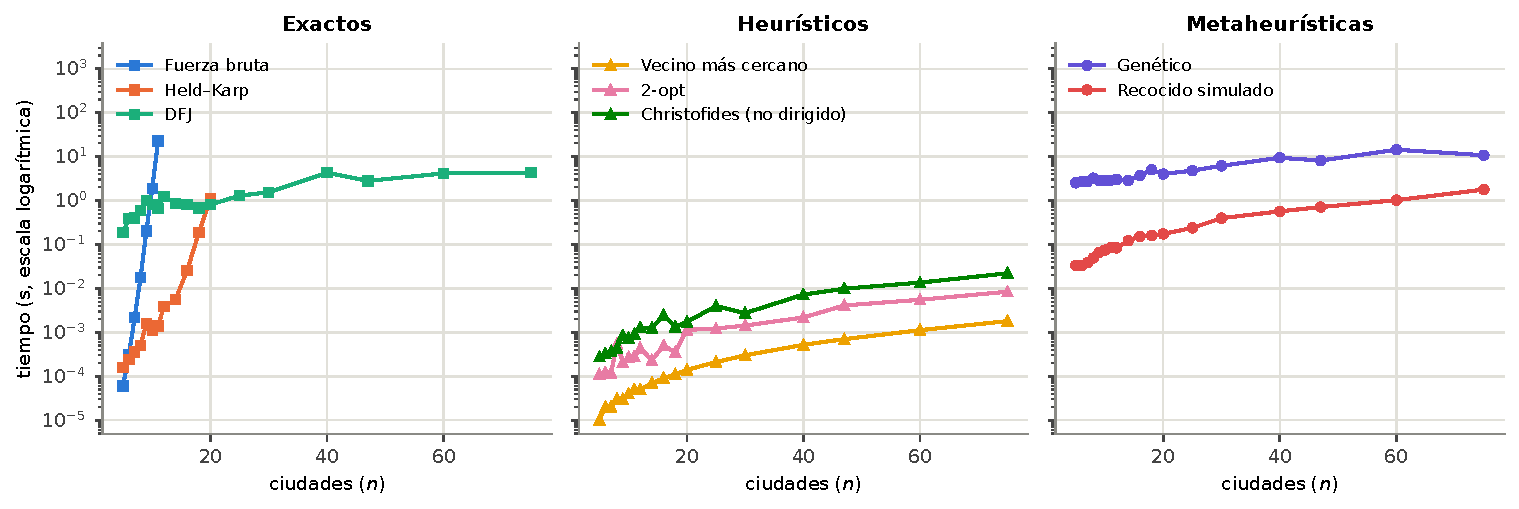
\includegraphics[width=\linewidth]{curvas_tiempo.pdf}
  \caption{Tiempo de cálculo frente al número de ciudades (escala logarítmica en el eje vertical). La fuerza bruta y Held--Karp se detienen en sus límites (11 y 20 ciudades).}
  \label{fig:tiempo}
\end{figure}

\begin{figure}[htbp]
  \centering
  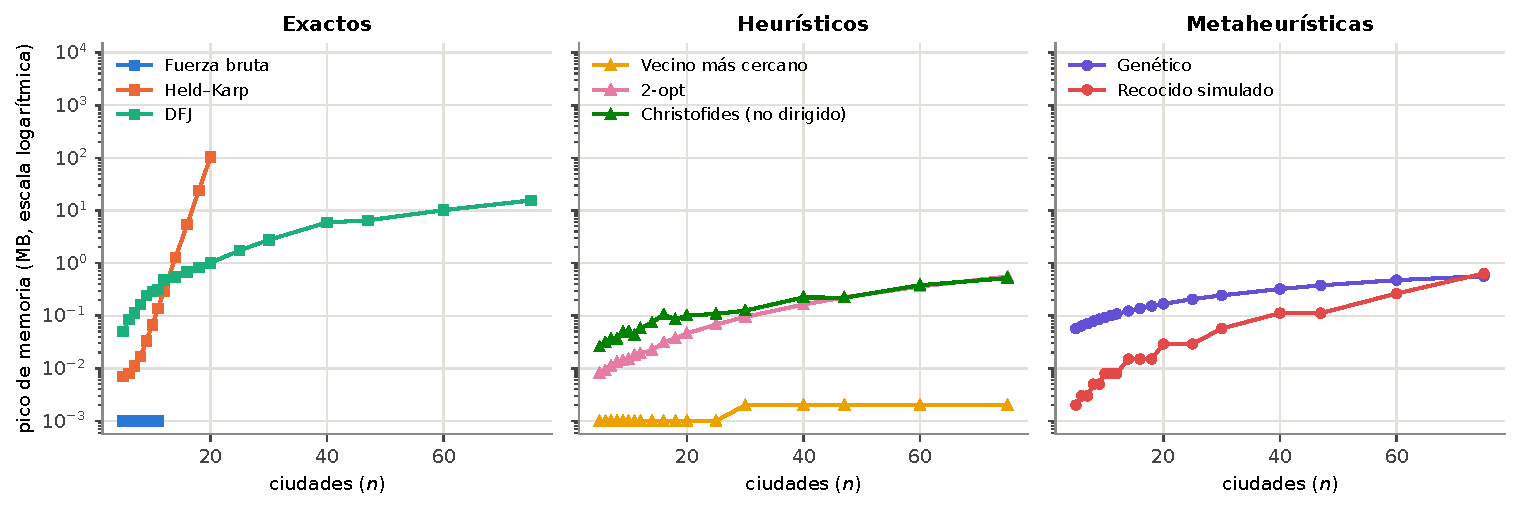
\includegraphics[width=\linewidth]{curvas_memoria.pdf}
  \caption{Pico de memoria reservada por Python frente al número de ciudades. La memoria de Held--Karp se duplica con cada ciudad.}
  \label{fig:memoria}
\end{figure}

\subsection{Complejidad en notación $O$: teoría frente a observación}

Para contrastar la complejidad teórica con la observada se ajustan los tiempos y la memoria medidos: un crecimiento exponencial $t\approx a\,b^{n}$ para los dos algoritmos de enumeración (donde $b$ es el factor por ciudad añadida) y una ley de potencias $t\approx a\,n^{k}$ para los demás
(ajuste lineal en escala logarítmica). El resultado se expresa en notación $O$ en la tabla~\ref{tab:bigo}.

\begin{table}[htbp]
  \centering
  \caption{Complejidad teórica y observada en notación $O$.}\label{tab:bigo}
  \footnotesize
  \begin{tabularx}{\linewidth}{@{}l X l X l@{}}
    \toprule
    Algoritmo & Tiempo (teoría) & Tiempo (observado) & Memoria (teoría) & Memoria (observada) \\
    \midrule
    Fuerza bruta & $O((n-1)!\cdot n)$ & $O(10{,}6^{\,n})$ & $O(n)$ & $\approx$ constante \\
    Held--Karp & $O(n^2\cdot 2^n)$ & $O(2{,}1^{\,n})$ & $O(n\cdot 2^n)$ & $O(2{,}1^{\,n})$ \\
    DFJ & $O(2^n)$ (peor caso) & $O(n)$ & $O(n^2)$ en la práctica & $O(n^{2})$ \\
    Vecino más cercano & $O(n^2)$ & $O(n^{1{,}9})$ & $O(n)$ & $\approx$ constante \\
    2-opt & $O(n^3)$ & $O(n^{1{,}8})$ & $O(n^2)$ & $O(n^{1{,}8})$ \\
    Christofides & $O(n^3)$ & $O(n^{1{,}6})$ & $O(n^2)$ & $O(n^{1{,}1})$ \\
    Recocido simulado & entre $O(n)$ y $O(n^2)$ & $O(n^{1{,}5})$ & $O(n^2)$ & $O(n^{2{,}1})$ \\
    Genético & $O(G\cdot P\cdot n\cdot q)$ & $O(n^{0{,}9})$ & $O(P\cdot n)$ & $O(n^{0{,}9})$ \\
    \bottomrule
  \end{tabularx}
\end{table}

Los dos algoritmos exactos de enumeración crecen de forma \textbf{exponencial}, en consonancia con la teoría: la fuerza bruta multiplica su tiempo por 10,6 con cada ciudad añadida ($R^2=1{,}00$; la teoría dice ``por $n$'', es decir, entre 9 y 11 en este rango) y Held--Karp por 2,1 ($R^2=0{,}96$; la
teoría dice aproximadamente 2), con una memoria que también se duplica por ciudad. El resto de algoritmos son \textbf{polinómicos}. El vecino más cercano ($n^{1,9}$) y el genético ($n^{0,9}$, lineal en $n$ por generación) coinciden con lo esperado; el 2-opt y Christofides salen con exponentes
menores que los teóricos, porque con 5 a 75 ciudades pesan los costes fijos y las operaciones vectorizadas de NumPy, y el exponente teórico se refiere al peor caso. DFJ es el caso más llamativo: su peor caso es exponencial, pero en estas instancias el tiempo crece apenas
de forma lineal (de 0,2~s con 5 ciudades a 4,3~s con 75).

Conviene recordar que la $O$ observada es una \emph{estimación} con tamaños de 5 a 75 ciudades y no una demostración.

\section{De enumerar a ser inteligente: la mejora entre algoritmos exactos}

La tabla~\ref{tab:exactos} compara el tiempo necesario para resolver al óptimo una instancia de $n$ ciudades con los tres algoritmos exactos (serie, grafo dirigido).

\begin{table}[htbp]
  \centering
  \caption{Tiempo (s) para resolver al óptimo una instancia de $n$ ciudades. «--» indica que el algoritmo no es aplicable.}\label{tab:exactos}
  \small
  \begin{tabular}{@{}r r r r@{\qquad}r r@{}}
    \toprule
    $n$ & Fuerza bruta & Held--Karp & DFJ & FB\,/\,HK & DFJ\,/\,HK \\
    \midrule
    8  & 0,018 & 0,0005 & 0,59 & 36 & 1.184 \\
    10 & 1,87 & 0,0011 & 0,82 & 1.641 & 747 \\
    11 & 22,5 & 0,0014 & 0,66 & 16.047 & 469 \\
    12 & -- & 0,0038 & 1,25 & -- & 328 \\
    14 & -- & 0,0056 & 0,85 & -- & 152 \\
    16 & -- & 0,026 & 0,82 & -- & 31,5 \\
    18 & -- & 0,18 & 0,68 & -- & 3,7 \\
    20 & -- & 1,10 & 0,81 & -- & 0,73 \\
    30 & -- & -- & 1,55 & -- & -- \\
    47 & -- & -- & 2,80 & -- & -- \\
    75 & -- & -- & 4,31 & -- & -- \\
    \bottomrule
  \end{tabular}
\end{table}

Held--Karp es \textbf{36 veces más rápido} que la fuerza bruta con 8 ciudades, \textbf{1.600 veces} con 10 y \textbf{16.000 veces} con 11. DFJ, en cambio, es \emph{más lento} que Held--Karp con pocas ciudades (el arranque del \emph{solver} cuesta entre 0,2 y 1~s: con 11 ciudades es 469 veces
más lento), pero \textbf{no tiene su pared}: las curvas se cruzan hacia las \textbf{20 ciudades} (0,81~s de DFJ frente a 1,10~s de Held--Karp), y DFJ resuelve 75 ciudades al óptimo en 4,3~s. En resumen: de 5 a 7 ciudades cualquiera sirve; de 8 a 19, Held--Karp; \textbf{desde 20, DFJ}.

\section{Calidad: cuánto se aleja del óptimo lo que no lo garantiza}

La tabla~\ref{tab:calidad} y la figura~\ref{fig:desviacion} muestran la desviación media respecto al óptimo de los algoritmos no exactos (estudio B; media de los subconjuntos y las semillas).

\begin{table}[htbp]
  \centering
  \caption{Desviación media respecto al óptimo (\%), por número de ciudades. Grafo dirigido, salvo Christofides (no dirigido).}\label{tab:calidad}
  \small
  \begin{tabular}{@{}r r r r r r@{}}
    \toprule
    $n$ & Vecino más cercano & Christofides & 2-opt & Recocido & Genético \\
    \midrule
    11 & 8,0 & 7,6 & 0,4 & 0,0 & 0,0 \\
    20 & 20,9 & 5,3 & 1,1 & 0,1 & 1,4 \\
    47 & 30,4 & 14,6 & 1,1 & 2,3 & 5,0 \\
    75 & 31,8 & 13,6 & 4,5 & 4,4 & 6,1 \\
    \bottomrule
  \end{tabular}
\end{table}

\begin{figure}[htbp]
  \centering
  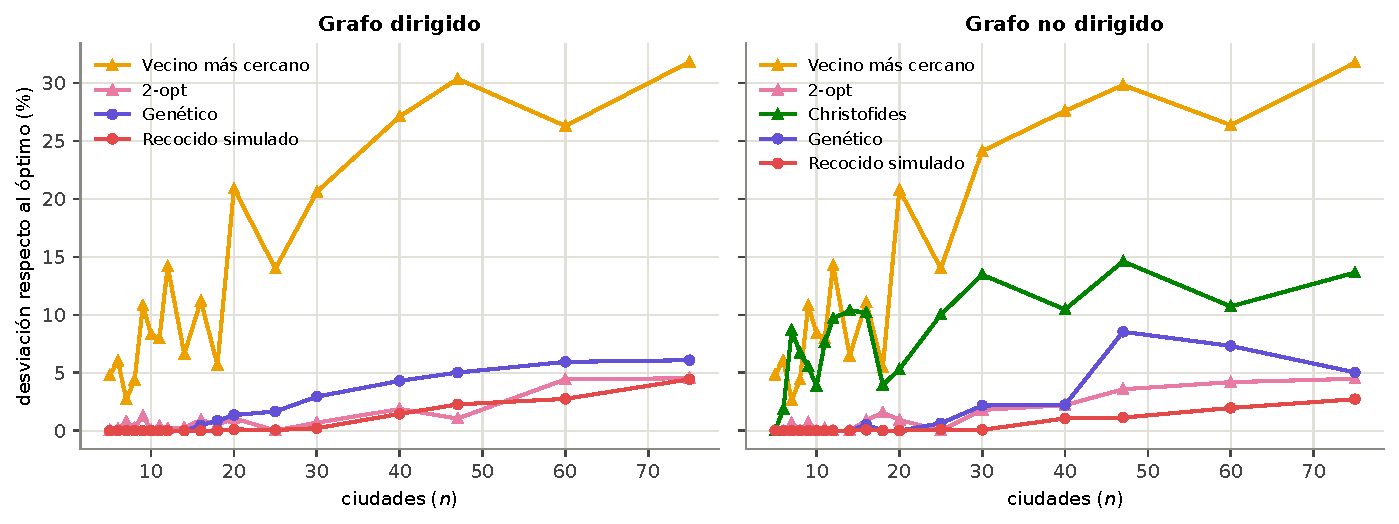
\includegraphics[width=0.92\linewidth]{desviacion.pdf}
  \caption{Desviación media respecto al óptimo (\%) en función del número de ciudades, en el grafo dirigido (izquierda) y no dirigido (derecha).}
  \label{fig:desviacion}
\end{figure}

\begin{itemize}
  \item El \textbf{vecino más cercano} es siempre el peor (entre un 3~\% y un 32~\% por encima del óptimo de media, hasta un 42~\% en un caso concreto) y empeora con el tamaño: solo sirve como punto de partida.
  \item \textbf{Christofides} cumple siempre su garantía (peor caso individual medido: +19,7~\%, muy por debajo del 50~\%), pero queda por encima del 2-opt: la garantía es un peor caso, no una predicción.
  \item El \textbf{2-opt} es el mejor equilibrio: con un error del 1--5~\% tarda milisegundos.
  \item \textbf{Recocido y genético llegan al óptimo hasta unas 14 ciudades} y después se alejan poco a poco. No mejoran al 2-opt en estos tamaños y tardan entre 170 y 2.000 veces más.
\end{itemize}

\subsection{Variabilidad de los algoritmos con azar}

Un solo resultado no describe a un algoritmo estocástico. Con 47 ciudades, el genético va del 1,0~\% al 8,3~\% de desviación (mediana 5,2~\%) y el recocido del 0,0~\% al 6,6~\% (mediana 2,2~\%); la figura~\ref{fig:dispersion} muestra cada ejecución.
Las medias esconden además casos malos: en la peor versión de toda España, el 2-opt llega a +18~\%, el recocido a +26~\% y el genético a +49~\%.

\begin{figure}[htbp]
  \centering
  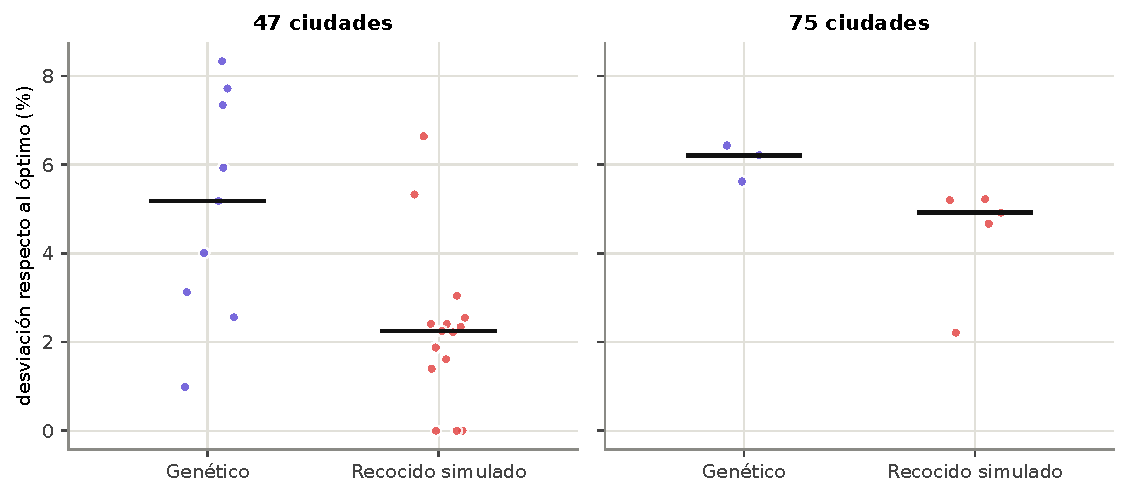
\includegraphics[width=0.7\linewidth]{dispersion.pdf}
  \caption{Desviación de cada ejecución del genético y del recocido simulado (grafo dirigido). La raya negra es la mediana.}
  \label{fig:dispersion}
\end{figure}

\section{Efecto de la versión del grafo}\label{sec:versiones_resultados}

Los resultados dependen tanto de la versión como del algoritmo. La figura~\ref{fig:rutas} muestra, para las 47 capitales, tres rutas sobre las carreteras reales.

\begin{figure}[htbp]
  \centering
  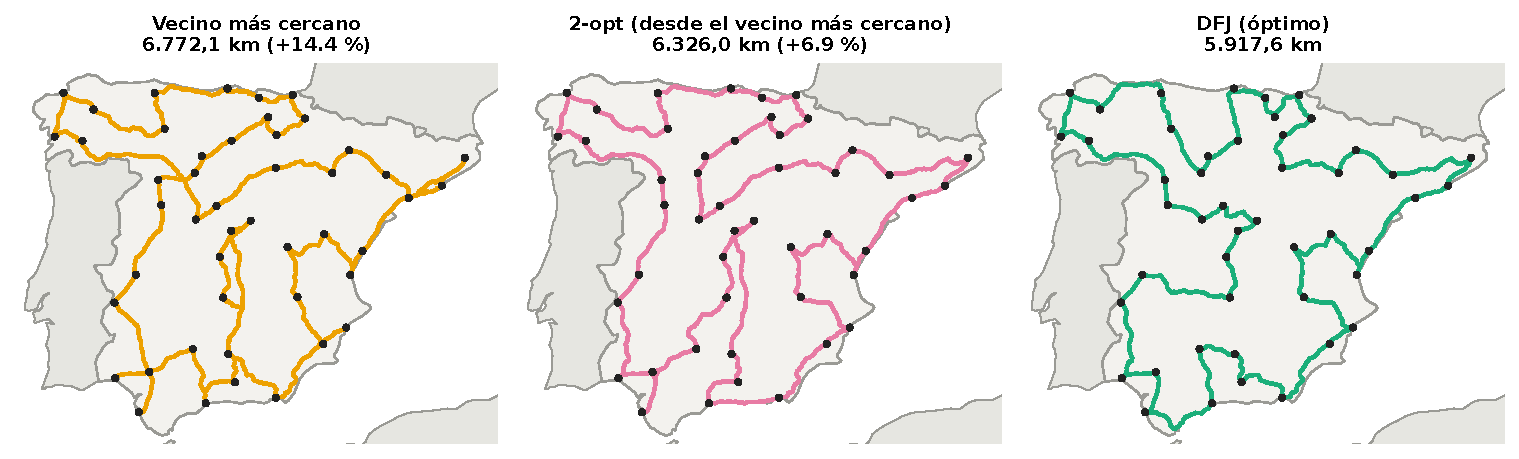
\includegraphics[width=\linewidth]{rutas_47.pdf}
  \caption{Rutas de las 47 capitales (versión \texttt{completo}/km, con sentidos únicos, saliendo de Madrid): vecino más cercano, 2-opt y óptimo (DFJ), dibujadas sobre el trazado de las carreteras.}
  \label{fig:rutas}
\end{figure}

\paragraph{Red de carreteras.} La tabla~\ref{tab:optimos} da el óptimo en cada versión de toda España. Sin autovías el óptimo cuesta un \textbf{30--38~\% más de kilómetros y casi el doble de tiempo} (+99~\% a +108~\%); con
\texttt{autovias\_principales}, solo un 3--4~\% más. Con \texttt{solo\_autovias} cuesta un 32--38~\% más de kilómetros y quedan fuera tres ciudades.

\paragraph{Sentido de las vías.} Ignorar los sentidos únicos apenas cambia el óptimo en la mayoría de las redes (0,7--4,0~\%), pero en \texttt{solo\_autovias} los sentidos cuestan un \textbf{13--19~\%}, porque en una red solo de autovías no se puede dar la vuelta.
Los heurísticos lo notan: con grafo dirigido el 2-opt se aleja de media un 6,9~\% (2,6~\% en no dirigido), el genético un 10,6~\% (4,3~\%) y el recocido un 5,2~\% (2,3~\%).

\paragraph{Calidad de los heurísticos según la red.} La tabla~\ref{tab:gapred} muestra la desviación media por red. \texttt{solo\_autovias} es la más difícil para los heurísticos (2-opt 8,1~\%, recocido 6,7~\%, genético 13,4~\%) y \texttt{sin\_autovias}, la mejor para el 2-opt (1,8~\%).

\begin{table}[htbp]
  \centering
  \caption{Óptimo (DFJ) en las versiones de toda España y coste respecto a la red completa (47 y 75 ciudades; con 44 y 72 en \texttt{solo\_autovias}).}\label{tab:optimos}
  \footnotesize
  \begin{tabular}{@{}l c r r r r@{}}
    \toprule
    & & \multicolumn{2}{c}{Óptimo en km} & \multicolumn{2}{c}{Óptimo en horas} \\
    \cmidrule(lr){3-4}\cmidrule(lr){5-6}
    Red & Ciudades & dirigido & no dirigido & dirigido & no dirigido \\
    \midrule
    \texttt{completo} & 47 & 5.917,6 & 5.875,3 & 63,3 & 62,2 \\
    & 75 & 6.146,2 & 6.069,8 & 67,7 & 65,9 \\
    \texttt{autovias\_principales} & 47 & 6.094,7 & 6.054,0 & 64,7 & 63,5 \\
    & 75 & 6.377,5 & 6.242,6 & 69,8 & 67,1 \\
    \texttt{sin\_autovias} & 47 & 7.661,4 & 7.573,7 & 125,7 & 123,8 \\
    & 75 & 8.465,7 & 8.331,4 & 140,6 & 137,4 \\
    \texttt{solo\_autovias} & 44 / 47 & 7.814,1 & 6.900,1 & 70,1 & 61,3 \\
    & 72 / 75 & 8.509,3 & 7.222,6 & 76,5 & 64,6 \\
    \bottomrule
  \end{tabular}
\end{table}

\begin{table}[htbp]
  \centering
  \caption{Desviación media (\%) de cada algoritmo en las 32 versiones de toda España, según la red de carreteras.}\label{tab:gapred}
  \small
  \begin{tabular}{@{}l r r r r@{}}
    \toprule
    Algoritmo & \texttt{completo} & \texttt{autovias\_principales} & \texttt{sin\_autovias} & \texttt{solo\_autovias} \\
    \midrule
    Vecino más cercano & 19,7 & 26,3 & 30,8 & 23,4 \\
    Christofides & 12,1 & 12,6 & 13,9 & 11,5 \\
    2-opt & 4,6 & 4,6 & 1,8 & 8,1 \\
    Recocido simulado & 2,9 & 2,7 & 2,7 & 6,7 \\
    Genético & 4,7 & 5,5 & 6,3 & 13,4 \\
    \bottomrule
  \end{tabular}
\end{table}

\paragraph{Kilómetros frente a tiempo.} La ruta más corta no es la más rápida. Para las 47 capitales, la ruta de mínimos kilómetros mide 5.917,6~km y tarda 64,5~h; la de mínimo tiempo mide 6.002,4~km y tarda 63,3~h. La ruta más rápida ahorra \textbf{1,2~h (1,9~\%)} a cambio de
\textbf{84,8~km (+1,4~\%)}, y las dos rutas comparten 31 de sus 47 tramos entre ciudades.

\section{Calidad frente a tiempo: ¿qué conviene usar?}

La figura~\ref{fig:calidad_tiempo} sitúa cada algoritmo según su tiempo (eje horizontal, logarítmico) y su desviación media (eje vertical): lo mejor está abajo y a la izquierda. Con 11 ciudades se comparan todos; con 75 los exactos de enumeración ya no caben.

\begin{figure}[htbp]
  \centering
  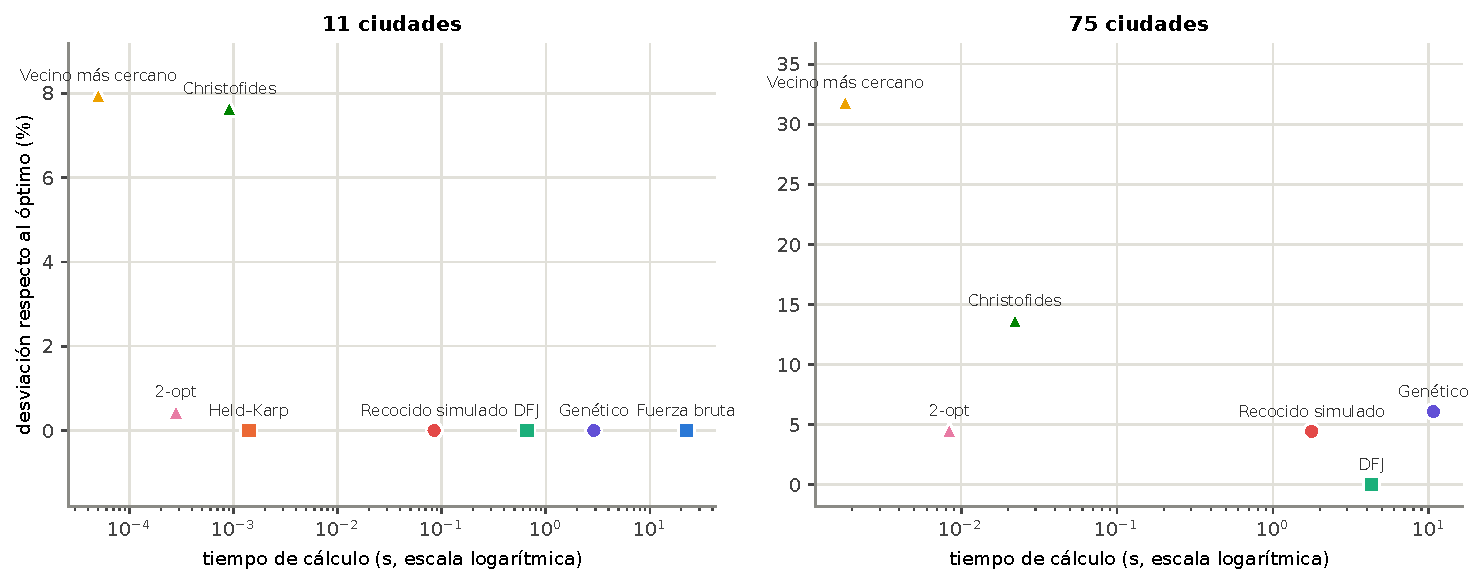
\includegraphics[width=\linewidth]{calidad_tiempo.pdf}
  \caption{Calidad frente a tiempo con 11 y con 75 ciudades (grafo dirigido; Christofides, no dirigido).}
  \label{fig:calidad_tiempo}
\end{figure}

\begin{table}[htbp]
  \centering
  \caption{Resumen con 47 y 75 ciudades (grafo dirigido): calidad, tiempo (serie) y memoria.}\label{tab:resumen}
  \small
  \begin{tabular}{@{}r l r r r r@{}}
    \toprule
    $n$ & Algoritmo & Desv. media (\%) & Peor (\%) & Tiempo (s) & Memoria (MB) \\
    \midrule
    47 & DFJ & 0,0 & 0,0 & 2,795 & 6,51 \\
    & 2-opt & 1,1 & 1,6 & 0,004 & 0,22 \\
    & Recocido simulado & 2,3 & 6,6 & 0,710 & 0,11 \\
    & Genético & 5,0 & 8,3 & 8,124 & 0,38 \\
    & Vecino más cercano & 30,4 & 36,1 & 0,001 & $<0{,}01$ \\
    \midrule
    75 & DFJ & 0,0 & 0,0 & 4,310 & 15,54 \\
    & Recocido simulado & 4,4 & 5,2 & 1,775 & 0,64 \\
    & 2-opt & 4,5 & 4,5 & 0,008 & 0,56 \\
    & Genético & 6,1 & 6,4 & 10,724 & 0,56 \\
    & Vecino más cercano & 31,8 & 31,8 & 0,002 & $<0{,}01$ \\
    \bottomrule
  \end{tabular}
\end{table}

\section{Cuánto distorsiona medir en paralelo}\label{sec:calibracion}

La calibración repitió en serie 15 tareas de la pasada en paralelo. El tiempo en paralelo resultó \textbf{2,46 veces mayor} de mediana, entre $\times 2{,}06$ (genético) y $\times 2{,}72$ (recocido simulado). Esto confirma que los tiempos solo son fiables en la pasada en serie, y justifica haber
medido los tiempos y la memoria de las curvas de complejidad en esa pasada.

\chapter{Conclusiones}\label{cap:conclusiones}

Este capítulo responde a las preguntas planteadas en la introducción, resume lo aprendido y recoge las limitaciones y el trabajo futuro.

\section{Respuestas a las preguntas del estudio}

\paragraph{P1. ¿Qué algoritmo se puede usar con qué versión?} Los tres algoritmos exactos y el resto de métodos no son intercambiables. La fuerza bruta solo sirve con 11 ciudades o menos y Held--Karp con 21 o menos, por lo que solo se pueden aplicar a las versiones regionales (4 a 13 ciudades)
y a subconjuntos pequeños; Christofides exige un grafo no dirigido. En las versiones de toda España (44 a 75 ciudades), el único exacto aplicable es DFJ. Los otros cinco algoritmos funcionan en las 240 versiones.

\paragraph{P2. ¿Cómo crecen el tiempo y la memoria?} Los exactos de enumeración crecen de forma exponencial, como predice la teoría: la fuerza bruta multiplica su tiempo por 10,6 con cada ciudad y se agota en 11 (22~s; con 13 serían unos 50 minutos); Held--Karp lo multiplica por 2,1 y su memoria $O(n\cdot 2^n)$ es el verdadero límite
(104~MB con 20 ciudades, inviable hacia las 21--22). Los demás algoritmos crecen de forma polinómica, con exponentes iguales o menores que los teóricos. DFJ, con un peor caso exponencial, resolvió las 75 ciudades al óptimo en 4,3~s.

\paragraph{P3. ¿Cuánto se pierde al renunciar al óptimo?} Con 75 ciudades, el vecino más cercano queda un 32~\% por encima del óptimo, Christofides un 14~\%, el 2-opt un 4,5~\%, el recocido un 4,4~\% y el genético un 6,1~\%. El 2-opt es el mejor equilibrio entre calidad y tiempo: con un 1--5~\% de error tarda milisegundos.
Los metaheurísticos llegan al óptimo con hasta unas 14 ciudades, pero con más no mejoran al 2-opt y tardan entre 170 y 2.000 veces más, además de variar entre ejecuciones.

\paragraph{P4. ¿Qué efecto tiene la versión del grafo?} Tanto como el algoritmo. Sin autovías, el óptimo cuesta un 30--38~\% más de kilómetros y casi el doble de tiempo. Con solo autovías, los sentidos únicos cuestan un 13--19~\%, porque no se puede dar la vuelta; en las demás redes ignorarlos apenas cambia el óptimo (0,7--4~\%).
Los heurísticos son menos robustos en grafos dirigidos y en la red más dispersa. Y la ruta más corta no es la más rápida: la de mínimo tiempo ahorra 1,2~h (1,9~\%) a cambio de 85~km más (+1,4~\%).

\paragraph{P5. ¿Qué conviene usar?} Depende del caso (tabla~\ref{tab:recomendaciones}).

\begin{table}[htbp]
  \centering
  \caption{Qué algoritmo usar en cada caso.}\label{tab:recomendaciones}
  \small
  \begin{tabularx}{\linewidth}{@{}X l X@{}}
    \toprule
    Si se quiere\dots & Usar & Notación $O$ y comportamiento \\
    \midrule
    El óptimo con hasta unas 19 ciudades & Held--Karp & $O(n^2\cdot 2^n)$ en tiempo y $O(n\cdot 2^n)$ en memoria: muy rápido, con un muro de memoria \\
    El óptimo con 20 o más ciudades & DFJ & exponencial en el peor caso, pero 4,3~s con 75 ciudades \\
    Una buena ruta en milisegundos & 2-opt & $O(n^2)$ por vuelta; 1--5~\% de error \\
    Una calidad garantizada & Christofides & $O(n^3)$; $\le 1{,}5\times$ el óptimo (solo grafo no dirigido) \\
    Explorar con azar & Recocido o genético & casi lineales en $n$, con un coste fijo alto y variabilidad entre ejecuciones \\
    Una ruta de partida & Vecino más cercano & $O(n^2)$; instantáneo, pero con un 3--32~\% de error \\
    \bottomrule
  \end{tabularx}
\end{table}

\section{Otras conclusiones}

\begin{itemize}
  \item \textbf{La garantía de Christofides es un peor caso, no una predicción.} Nunca superó el +20~\%, muy por debajo del +50~\% garantizado, pero queda por encima del 2-opt, que no ofrece ninguna garantía. Su valor está en la seguridad, no en la calidad media.
  \item \textbf{Una metaheurística bien ajustada importa.} La primera versión del genético, con mutaciones aleatorias simples, se quedaba entre un 19~\% y un 37~\% por encima del óptimo; añadir una pequeña búsqueda local en la mutación lo bajó al 2--5~\%.
  \item \textbf{Lo que se mide depende de cómo se mide.} En paralelo, los tiempos salen unas 2,5 veces más lentos; por eso los costes salen de una pasada y los tiempos de otra. Y contrastar tres algoritmos exactos independientes dio cero discrepancias y descubrió dos fallos que las pruebas por separado no habían encontrado.
  \item \textbf{Un buen conjunto de datos es una parte del resultado.} Obtener un grafo vial fiable y justificar las versiones del problema ocupó una parte considerable del trabajo y condiciona todo lo demás.
\end{itemize}

\section{Limitaciones}

Los metaheurísticos se midieron con sus parámetros por defecto y pocas semillas (3 y 5); con 75 ciudades solo hay un subconjunto (el conjunto completo); la memoria de DFJ no cuenta la del \emph{solver} CBC; y los tamaños llegan a 75 ciudades, donde DFJ sigue siendo inmediato.
Con muchas más ciudades es probable que DFJ deje de serlo y los metaheurísticos pasen a ser la mejor opción, pero no se ha medido. Además, las distancias son de coche y no consideran tráfico, peajes ni obras, y las coordenadas de las ciudades proceden de OpenStreetMap y no de una fuente oficial.

\section{Trabajo futuro}

\begin{itemize}
  \item Ajustar los parámetros del recocido y del genético a cada tamaño, y probar variantes más potentes (por ejemplo, búsqueda local de tipo Or-opt o Lin--Kernighan).
  \item Probar instancias de cientos o miles de ciudades, donde DFJ deja de ser inmediato, y comparar con soluciones de referencia como Concorde.
  \item Realizar el estudio de escala por comunidades autónomas con las versiones regionales, y ampliar el conjunto de ciudades a municipios más pequeños.
  \item Añadir restricciones realistas: ventanas horarias, peajes, tráfico o límites de jornada, y pasar de un único viajante a varios vehículos.
  \item Ampliar la web con un panel de resultados del estudio y un recorrido guiado del proyecto.
\end{itemize}

\chapter{La web interactiva}\label{cap:web}

\section{Propósito}

Los algoritmos del viajante son más fáciles de entender viéndolos funcionar que leyendo su pseudocódigo. Por eso, además del estudio, se ha construido una \textbf{web interactiva} que anima los ocho algoritmos sobre el mapa de España, con la ruta construyéndose
paso a paso sobre las carreteras reales. Sirve como apoyo visual para la presentación del trabajo y puede quedar publicada de forma permanente.

\section{Qué ofrece}

La web tiene tres vistas:
\begin{description}[leftmargin=0pt,labelindent=0pt,style=nextline]
  \item[Laboratorio.] Se elige un algoritmo, un conjunto de ciudades (pulsando sobre el mapa o la lista, o con ejemplos predefinidos de 6, 9, 13, 47 y 75 ciudades), la medida (kilómetros o tiempo) y si se respetan los sentidos únicos. Un reproductor permite ejecutar, pausar, avanzar y retroceder
        paso a paso, saltar al resultado final y cambiar la velocidad. Junto al mapa aparecen el \textbf{pseudocódigo con la línea actual resaltada}, una \textbf{explicación en lenguaje llano} de lo que ocurre en cada paso, el coste de la ruta actual y de la mejor encontrada, una gráfica de la evolución del coste y la ficha del algoritmo.
  \item[Carrera.] Varios algoritmos resuelven \emph{a la vez} las mismas ciudades. Cada uno avanza durante el mismo tiempo de cálculo, de modo que el que termina antes es de verdad el más rápido. Al final aparece una tabla con el coste, la desviación frente al mejor y el tiempo de cálculo.
        Los algoritmos no aplicables se descartan con su motivo, igual que en el estudio.
  \item[Acerca de.] Explica qué es la web y cómo se usa.
\end{description}
Hay tema oscuro (mapa nocturno, pensado para proyector) y claro, botón de pantalla completa, zoom con la rueda del ratón y atajos de teclado.

\begin{figure}[htbp]
  \centering
  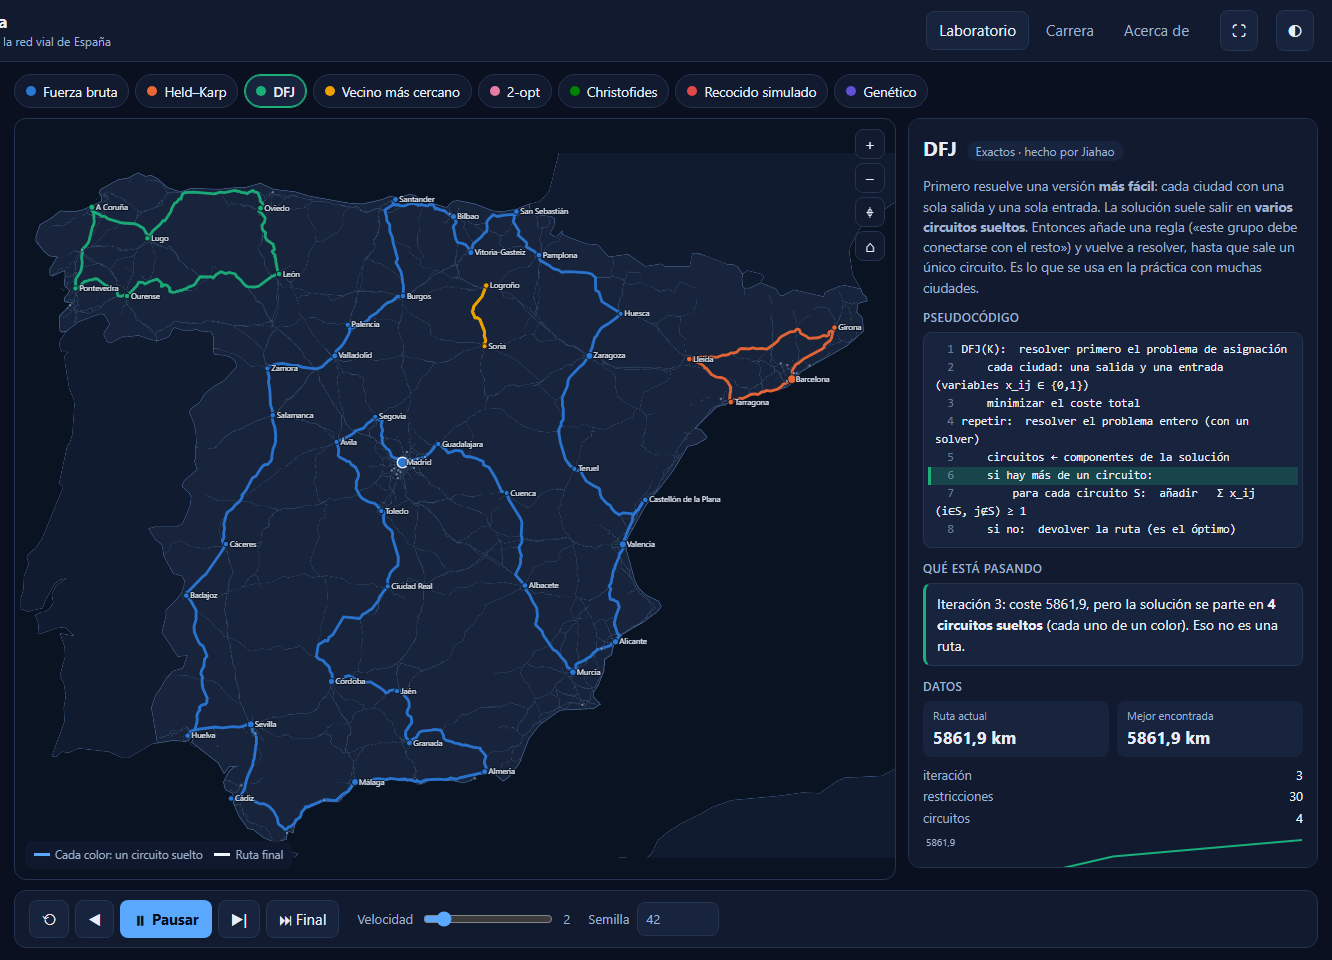
\includegraphics[width=0.97\linewidth]{web_05_dfj_circuitos_sueltos.png}
  \caption{Laboratorio: DFJ con las 47 capitales. La primera solución del problema de asignación se parte en varios circuitos sueltos (cada uno de un color) sobre las carreteras reales; el pseudocódigo resalta el paso actual.}
  \label{fig:web_dfj}
\end{figure}

\begin{figure}[htbp]
  \centering
  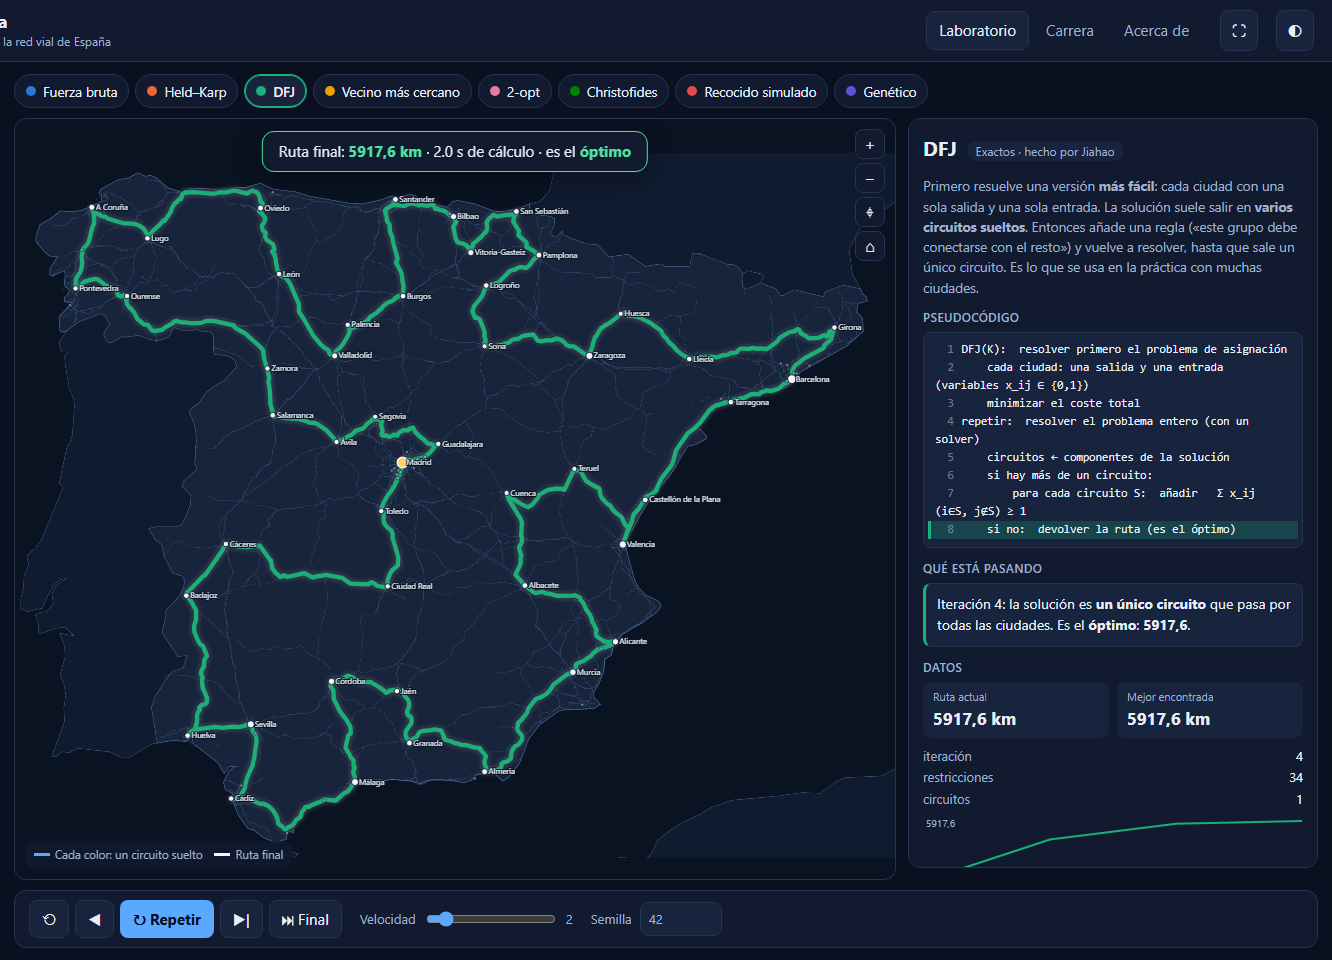
\includegraphics[width=0.97\linewidth]{web_06_dfj_optimo_47_capitales.png}
  \caption{Laboratorio: ruta óptima de las 47 capitales (5.917,6~km) encontrada por DFJ tras cuatro iteraciones.}
  \label{fig:web_optimo}
\end{figure}

\begin{figure}[htbp]
  \centering
  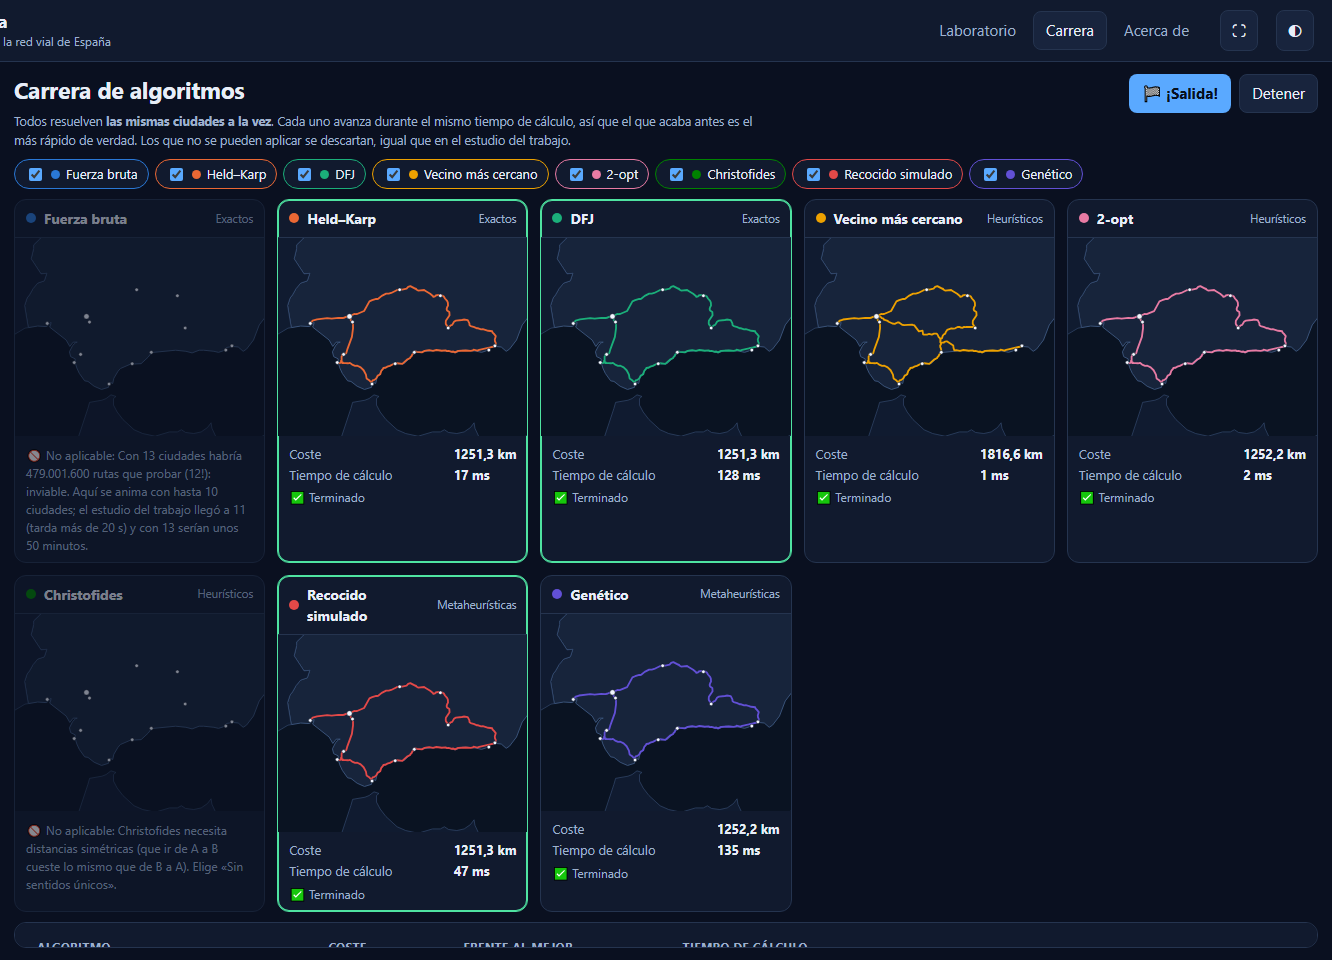
\includegraphics[width=0.97\linewidth]{web_10_carrera.png}
  \caption{Carrera de algoritmos sobre las 13 ciudades de Andalucía. Fuerza bruta y Christofides se descartan con su motivo; Held--Karp, DFJ y el recocido encuentran el óptimo (1.251,3~km) en 17, 128 y 47~ms.}
  \label{fig:web_carrera}
\end{figure}

\section{Cómo está hecha}

\begin{itemize}
  \item \textbf{Sin servidor.} Todo se calcula en el navegador, con JavaScript. Cada algoritmo está escrito como un \emph{generador} en el que cada paso emite un «fotograma» (ruta, aristas resaltadas, línea de pseudocódigo, explicación y coste),
        lo que permite reproducir, pausar y retroceder con el mismo código.
  \item \textbf{Mapa.} Un mapa esquemático propio (contorno de la península y países vecinos, y red de autovías y vías rápidas de fondo) dibujado con \emph{canvas} y SVG, con zoom y desplazamiento.
  \item \textbf{Carreteras reales.} Para cada par de las 75 ciudades se ha precalculado, con el grafo del trabajo, el camino mínimo y se ha guardado su trazado simplificado y codificado (1,1~MB para 2.775 pares); las rutas se dibujan siguiendo esas carreteras.
  \item \textbf{Solucionadores.} DFJ usa \emph{HiGHS}~\cite{huangfu2018}, un \emph{solver} de programación entera compilado a WebAssembly, y Christofides usa el emparejamiento de Edmonds; ambas librerías (licencia MIT) se incluyen en el repositorio, de modo que la web funciona sin internet.
  \item \textbf{Datos.} Las distancias son las mismas tablas del trabajo (capítulo~\ref{cap:versiones}).
\end{itemize}

\section{Cómo sabemos que es correcta}

Los algoritmos de JavaScript se contrastan automáticamente con los resultados de Python: fuerza bruta, Held--Karp y DFJ dan el mismo óptimo (5.917,562~km con las 47 capitales, 460,438~km en Galicia, 1.251,307~km en Andalucía y 6.146,165~km con las 75 ciudades);
el vecino más cercano y el 2-opt dan los mismos costes que en Python (6.772,1~km y 6.326,0~km con las 47 capitales); y Christofides, el genético y el recocido devuelven rutas válidas con costes dentro de lo esperado. Además se probaron las vistas con un navegador automatizado, sin errores de consola.

\section{Publicación}

La web es una carpeta del repositorio (\texttt{web/}) que se abre en local con un servidor sencillo (doble clic en \texttt{iniciar\_web.bat} o \texttt{python -m http.server}). El repositorio incluye además una acción de GitHub que la publica en \emph{GitHub Pages} cuando
el propietario del repositorio la activa, de modo que queda en una dirección permanente. La guía de uso (documento aparte) explica el manejo paso a paso.

\chapter{Organización del trabajo, uso de IA y lecciones aprendidas}\label{cap:organizacion}

\section{Reparto del trabajo}

El trabajo lo realizan cuatro personas (tabla~\ref{tab:equipo}). La construcción del grafo, las versiones, las herramientas de integración, el estudio empírico, la web y esta memoria las llevó Raimundo, que también coordinó al resto; los demás aportaron un algoritmo cada uno como mínimo
(Raimundo, cuatro). El reparto de algoritmos se acordó en el grupo, y a cada persona se le asignó trabajar en su propia rama del repositorio.

\begin{table}[htbp]
  \centering
  \caption{Autoría de cada parte del trabajo.}\label{tab:equipo}
  \small
  \begin{tabularx}{\linewidth}{@{}l X@{}}
    \toprule
    Persona & Contribución \\
    \midrule
    Raimundo & Partes 1, 2, 4 y 5; Held--Karp, 2-opt, Christofides y genético; herramientas de integración; Anexo~C; web; memoria y guía de uso; coordinación. \\
    Pablo & Fuerza bruta y vecino más cercano. \\
    Jiahao & DFJ (programación entera con restricciones de subciclo). \\
    Juan & Recocido simulado (MCMC). \\
    \bottomrule
  \end{tabularx}
\end{table}

\section{Flujo de trabajo con GitHub}

El código se versiona en un repositorio de GitHub. Cada persona trabaja en su rama (\texttt{dev-pablo}, \texttt{dev\_jiahao}, \texttt{dev\_juan}, \texttt{dev-raimundo}) y entrega mediante \emph{Pull Request} hacia la rama principal. Para evitar conflictos de git con un solo
\emph{notebook} compartido, cada algoritmo se programa en su \textbf{propio \emph{notebook}} dentro de \texttt{parte3/}, a partir de una plantilla que ya contiene el código de preparación (la carga de las versiones del grafo). Una herramienta (\texttt{herramientas.py}) hace tres cosas:
regenerar la plantilla a partir del \emph{notebook} principal, \emph{unificar} el formato de todos los \emph{notebooks} (ficha, kernel, cabecera de pruebas) e \emph{integrar} automáticamente los algoritmos en el \emph{notebook} principal, de forma repetible. Todos los \emph{notebooks} siguen la misma estructura:
título, ficha (autor, tipo, complejidad, límite práctico), teoría, código, pruebas y resultados. Los datos de las fichas están en un único archivo (\texttt{fichas.json}), que alimenta también la tabla comparativa del \emph{notebook} y las etiquetas de la web.
Una guía (\texttt{CONTRIBUTING.md}) explica el proceso a los compañeros.

\section{Uso de herramientas de inteligencia artificial}

En el trabajo se ha usado \textbf{Claude Code} (Anthropic), un asistente de programación con modelos de lenguaje, para algunas partes. Para que el uso sea transparente, se registra qué se hizo con él (tabla~\ref{tab:ia}). En todos los casos, el código y los resultados se ejecutaron y comprobaron antes de incorporarlos,
y las pruebas de contraste entre algoritmos (capítulo~\ref{cap:resultados}) refuerzan esa comprobación.

\begin{table}[htbp]
  \centering
  \caption{Uso de IA en el trabajo.}\label{tab:ia}
  \small
  \begin{tabularx}{\linewidth}{@{}>{\raggedright\arraybackslash}p{0.34\linewidth} l X@{}}
    \toprule
    Parte & Herramienta & Para qué \\
    \midrule
    Partes 1, 2 y 4; herramientas de integración; Anexo~C; guía del equipo & Claude Code & Escribir y probar los \emph{scripts} de descarga y construcción del grafo, el código del \emph{notebook}, la plantilla, el estudio y su análisis. \\
    Held--Karp, 2-opt, Christofides y genético & Claude Code & Teoría, código, pruebas y redacción de resultados; contrastados con la fuerza bruta y con DFJ. \\
    Web interactiva y esta memoria & Claude Code & Programación de la web, generación de figuras y redacción, a partir de los datos y resultados del estudio. \\
    Fuerza bruta, vecino más cercano (Pablo); DFJ (Jiahao); recocido simulado (Juan) & \multicolumn{2}{>{\raggedright\arraybackslash}p{0.60\linewidth}}{Cada autor debe indicar en \texttt{REGISTRO.md} y en su ficha el uso de IA que haya hecho.} \\
    \bottomrule
  \end{tabularx}
\end{table}

\section{Problemas encontrados y lecciones aprendidas}\label{sec:problemas}

Un trabajo de este tamaño no sale a la primera. Estos son los problemas más relevantes, cómo se resolvieron y qué enseñan:
\begin{itemize}
  \item \textbf{La API Overpass no escalaba.} Solo se completó el 6~\% de la descarga en once horas. Lección: para datos masivos, descargar un extracto y filtrarlo en local; ganó reproducibilidad (sección~\ref{sec:construccion}).
  \item \textbf{Falta de memoria al construir el grafo.} El flujo estándar necesitaba unos 12~GB. Lección: reescribir la simplificación con \emph{arrays} (2,2~GB de pico), comprobando contra el grafo anterior que el resultado era idéntico.
  \item \textbf{Ejecuciones largas interrumpidas por falta de memoria.} Dos veces el sistema detuvo ejecuciones del \emph{notebook} completo por memoria. Lección: dejar el equipo libre, y diseñar el estudio para que guarde cada resultado al llegar y se pueda reanudar.
  \item \textbf{Un algoritmo exacto dependía de la versión de una librería} (la de programación entera, PuLP, devuelve cosas distintas según la versión). Se escribió de forma compatible y se añadió la dependencia a los requisitos.
  \item \textbf{Dos fallos con grafos no dirigidos} (recocido simulado y DFJ) que solo apareció al ejecutar sistemáticamente todos los algoritmos sobre todas las versiones. Lección: probar cada algoritmo sobre \emph{todos} los tipos de entrada que admite su contrato; el estudio sirvió también de prueba.
  \item \textbf{El paralelismo distorsiona los tiempos} unas 2,5 veces en el equipo usado. Lección: separar lo que no depende de la carga (costes) de lo que sí (tiempos), medidos en dos pasadas.
  \item \textbf{Cifras que no coincidían con lo medido.} En algún \emph{notebook} un texto afirmaba tiempos o errores distintos de los que salían al ejecutarlo; se sustituyeron por las cifras medidas. Lección: generar las tablas de resultados a partir de la ejecución, no a mano.
\end{itemize}

\section{Reproducibilidad}

Todo se puede rehacer con los comandos del apéndice~\ref{ap:reproducir}: descargar el extracto y construir el grafo (unos 11 minutos), recalcular las tablas de distancias (unos 2 minutos), ejecutar el estudio completo (unos 60 minutos) y regenerar las figuras. El grafo grande no se guarda en el repositorio (supera el límite de 100~MB de
GitHub), pero las tablas de distancias, los resultados del estudio y los datos de la web sí, de modo que quien programa un algoritmo o usa la web no necesita el grafo.

\appendix\apendicestyle
\chapter{Reproducir el trabajo}\label{ap:reproducir}

Desde la carpeta del proyecto y con las dependencias instaladas (\texttt{pip install -r requirements.txt}):

\begin{lstlisting}
# 1. Descargar el extracto de OpenStreetMap y construir el grafo (anexos A y B)
python anexos/descargar_red.py          # ~1,4 GB, ~7 min, reanudable
python anexos/construir_grafo.py        # ~4 min, ~2,3 GB de RAM

# 2. Abrir el notebook (el trabajo): partes 1 a 5
jupyter lab trabajo_tsp.ipynb           # las tablas de distancias ya estan en data/versiones/

# 3. Repetir el estudio empirico (anexo C)
python anexos/ejecutar_estudio.py       # en paralelo, ~42 min
python anexos/ejecutar_estudio.py --serie   # tiempos y memoria, ~15 min (equipo en reposo)

# 4. Regenerar las figuras y compilar esta memoria
python memoria/figuras/generar_figuras.py
cd memoria && tectonic -X compile memoria.tex

# 5. Abrir la web
web/iniciar_web.bat                     # o: python -m http.server 8000 (dentro de web/)
\end{lstlisting}

Si solo se van a programar o probar algoritmos, no hace falta el grafo grande ni los anexos: las versiones ya están calculadas en \texttt{data/versiones/}, y basta con abrir el \emph{notebook}, saltar la Parte~1 y ejecutar desde la Parte~2.

\chapter{Estructura del repositorio}\label{ap:estructura}

\begin{table}[htbp]
  \centering
  \caption{Contenido del repositorio.}
  \small
  \begin{tabularx}{\linewidth}{@{}l X@{}}
    \toprule
    Ruta & Contenido \\
    \midrule
    \texttt{trabajo\_tsp.ipynb} & El trabajo: \emph{notebook} principal con las cinco partes. \\
    \texttt{anexos/} & Anexo~A (descarga), Anexo~B (construcción del grafo) y Anexo~C (estudio empírico). \\
    \texttt{parte3/} & Un \emph{notebook} por algoritmo, plantilla, \texttt{fichas.json} y \texttt{herramientas.py}. \\
    \texttt{data/ciudades.csv} & Las 75 ciudades (nombre, coordenadas, población, comunidad). \\
    \texttt{data/versiones/} & 16 tablas de distancias y catálogo de las 480 versiones. \\
    \texttt{data/resultados/} & Resultados del estudio empírico (archivos CSV). \\
    \texttt{web/} & La web interactiva (código, datos, librerías, pruebas y capturas). \\
    \texttt{memoria/} & Esta memoria (fuente \LaTeX\ y figuras) y su generador de figuras. \\
    \texttt{guia/} & La guía de uso (fuente \LaTeX). \\
    \texttt{README.md}, \texttt{REGISTRO.md}, \texttt{CONTRIBUTING.md} & Documentación del proyecto, registro de autoría y uso de IA, y guía para colaborar. \\
    \bottomrule
  \end{tabularx}
\end{table}

\chapter{Fuentes y licencias}\label{ap:licencias}

\begin{itemize}
  \item \textbf{Carreteras:} \textcopyright\ colaboradores de OpenStreetMap, bajo licencia ODbL; extracto de España de Geofabrik (\texttt{spain-latest.osm.pbf}, 19 de octubre de 2026).
  \item \textbf{Ciudades y población:} INE, \emph{Cifras oficiales de población de los municipios españoles: Revisión del Padrón Municipal}, a 1 de enero de 2025 (BOE-A-2025-25362). Las coordenadas proceden de nodos de OpenStreetMap.
  \item \textbf{Contornos del mapa de la web:} Natural Earth (dominio público), a través del paquete \texttt{world-atlas}.
  \item \textbf{Librerías de la web:} HiGHS (\texttt{highs-js}) y \texttt{edmonds-blossom}, ambas con licencia MIT, incluidas en \texttt{web/vendor/}.
\end{itemize}

\clearpage
\addcontentsline{toc}{chapter}{Bibliografía}
\markboth{Bibliografía}{}
\begin{thebibliography}{99}
\small\setlength{\itemsep}{0.2em}
\bibitem{applegate2006} D.~L. Applegate, R.~E. Bixby, V. Chvátal y W.~J. Cook. \emph{The Traveling Salesman Problem: A Computational Study}. Princeton University Press, 2006.
\bibitem{bellman1962} R. Bellman. Dynamic programming treatment of the travelling salesman problem. \emph{Journal of the ACM}, 9(1):61--63, 1962.
\bibitem{boeing2017} G. Boeing. OSMnx: New methods for acquiring, constructing, analyzing, and visualizing complex street networks. \emph{Computers, Environment and Urban Systems}, 65:126--139, 2017.
\bibitem{christofides1976} N. Christofides. Worst-case analysis of a new heuristic for the travelling salesman problem. Informe técnico 388, Graduate School of Industrial Administration, Carnegie Mellon University, 1976.
\bibitem{croes1958} G.~A. Croes. A method for solving traveling-salesman problems. \emph{Operations Research}, 6(6):791--812, 1958.
\bibitem{davis1985} L. Davis. Applying adaptive algorithms to epistatic domains. En \emph{Proceedings of the 9th International Joint Conference on Artificial Intelligence (IJCAI)}, pp.\ 162--164, 1985.
\bibitem{dfj1954} G. Dantzig, R. Fulkerson y S. Johnson. Solution of a large-scale traveling-salesman problem. \emph{Operations Research}, 2(4):393--410, 1954.
\bibitem{dijkstra1959} E.~W. Dijkstra. A note on two problems in connexion with graphs. \emph{Numerische Mathematik}, 1:269--271, 1959.
\bibitem{edmonds1965} J. Edmonds. Paths, trees, and flowers. \emph{Canadian Journal of Mathematics}, 17:449--467, 1965.
\bibitem{garey1979} M.~R. Garey y D.~S. Johnson. \emph{Computers and Intractability: A Guide to the Theory of NP-Completeness}. W.~H. Freeman, 1979.
\bibitem{hagberg2008} A.~A. Hagberg, D.~A. Schult y P.~J. Swart. Exploring network structure, dynamics, and function using NetworkX. En \emph{Proceedings of the 7th Python in Science Conference (SciPy 2008)}, pp.\ 11--15, 2008.
\bibitem{haklay2008} M. Haklay y P. Weber. OpenStreetMap: User-generated street maps. \emph{IEEE Pervasive Computing}, 7(4):12--18, 2008.
\bibitem{harris2020} C.~R. Harris et~al. Array programming with NumPy. \emph{Nature}, 585:357--362, 2020.
\bibitem{heldkarp1962} M. Held y R.~M. Karp. A dynamic programming approach to sequencing problems. \emph{Journal of the Society for Industrial and Applied Mathematics}, 10(1):196--210, 1962.
\bibitem{holland1975} J.~H. Holland. \emph{Adaptation in Natural and Artificial Systems}. University of Michigan Press, 1975.
\bibitem{huangfu2018} Q. Huangfu y J.~A.~J. Hall. Parallelizing the dual revised simplex method. \emph{Mathematical Programming Computation}, 10:119--142, 2018.
\bibitem{karp1972} R.~M. Karp. Reducibility among combinatorial problems. En R.~E. Miller y J.~W. Thatcher (eds.), \emph{Complexity of Computer Computations}, pp.\ 85--103. Plenum Press, 1972.
\bibitem{kirkpatrick1983} S. Kirkpatrick, C.~D. Gelatt y M.~P. Vecchi. Optimization by simulated annealing. \emph{Science}, 220(4598):671--680, 1983.
\bibitem{metropolis1953} N. Metropolis, A.~W. Rosenbluth, M.~N. Rosenbluth, A.~H. Teller y E. Teller. Equation of state calculations by fast computing machines. \emph{The Journal of Chemical Physics}, 21(6):1087--1092, 1953.
\bibitem{virtanen2020} P. Virtanen et~al. SciPy 1.0: fundamental algorithms for scientific computing in Python. \emph{Nature Methods}, 17:261--272, 2020.
\end{thebibliography}

\end{document}
